% Size of page, document
\documentclass[11pt, titlepage, a4paper]{article}
\usepackage[left=1.5cm,text={17cm, 24cm},top=3cm,left=2cm]{geometry}

% Images
\usepackage{graphicx}

% Pseudo-code
\usepackage{amsmath}
\usepackage{algorithm}
\usepackage[noend]{algpseudocode}

% UTF-8; Czech
\usepackage[czech]{babel}
\usepackage[utf8]{inputenc}

% citations
\usepackage{url}

\graphicspath{ {./experiments/} }

\makeatletter
\def\BState{\State\hskip-\ALG@thistlm}
\makeatother

\title{IMS - Celulární automaty}

\author{
    Vašíček, Ondřej\\
    \texttt{xvasic25@stud.fit.vutbr.cz}
    \and
    Kočica, Filip\\
    \texttt{xkocic01@stud.fit.vutbr.cz}
}

% table of contents depth limit
\setcounter{tocdepth}{2}

\begin{document}

\maketitle

\tableofcontents
\newpage

\section{Úvod}
Tato studie je zaměřena na simulaci evakuace osob z~budov typu~L (komplexní, obsahující množství překážek)~\cite{source_CA} za účelem nalezení optimálního množství evakuačních východů a jejich rozmístění. Evakuace osob je problematika, se kterou se reálně těžko experimentuje, jelikož k~experimentu je potřeba velké množství osob a reálný model prostředí. Z~časových i zdrojových důvodů umožňuje simulace provést výrazně větší množství experimentů a zároveň umožňuje experimentovat s~libovolným množstvím variant rozmístění východů. Pohyb osob během evakuace je modelován pomocí celulárního automatu a používá řadu vlivů pro výpočet směru dalšího pohybu osoby. K~simulaci jsme přidali šíření ohně a jeho vliv na pohyb osob během evakuace. To umožňuje rozložení východů hodnotit i z~pohledu vzniku "slepých" uliček, ve kterých můžou být osoby ohněm odříznuty od východů.


    \subsection{Autoři a zdroje}
    Autory simulačního nástroje prezentovaného v~této simulační studii jsou Ondřej Vašíček a Filip Kočica. Nástroj byl implementován na základě modelu prezentovaného v~článku \textit{Cellular Automata Evacuation Model Considering Information Transfer in Building with Obstacles}~\cite{source_CA}. Z~tohoto článku byl převzat výpočet změny stavů buněk celulárního automatu určující pohyb osob na základě dynamických a statických vlivů okolí. Dále jsme převzali rozložení osob, překážek a východů pro základní experimenty~(kino sál). Článek také simulaci rozšiřuje o~přenos informací formou tabulí na křižovatkách, které určují kterým směrem mají osoby odbočit podle obsazenosti jednotlivých východů. Toto rozšíření jsme do našeho nástroje neimplementovali, protože odbočuje od čistého celulárního automatu a taky simulaci omezuje na jedno konkrétní rozložení východů a uliček mezi nimi. Jako základ nastudování celulárních automatů jsme použili přednášky předmětu IMS~\cite{IMS}

    \subsection{Experimentální ověření validity}
    Žádné experimentální ověření validity modelu v~reálném světě neproběhlo, protože koncepty použité pro simulaci jsme převzali z~článku tak, jak bylo určeno variantou zadání. Reálně experimentovat s~evakuací osob by pro nás bylo také velmi náročné (v~případě kina snad nemožné). Ověření validity pomocí simulačního modelu proběhlo skrze řadu experimentů testujících jednotlivé modelované vlivy pohybu osob s~různými parametry simulace. Tyto experimenty jsou uvedeny v~sekci~\ref{test_experiments}.

\section{Rozbor tématu a použitých metod/technologií}
\label{rozbor_tematu_a_pouzitych_metod}
Pohyb osob během evakuace se do určité míry jeví stochasticky. Osoby se sice pohybují celkově směrem k~některému východu, avšak konkrétní cesta, kterou si osoba zvolí, je kombinací velkého množství faktorů včetně individuální osobnosti jedince. Pohyb osob lze tedy celkově považovat za pohyb směrem k~některému z~východů (nejbližšímu nebo nejznámějšímu)~\cite{source_CA}. Osoby mají dále tendenci pohybovat se spíše velkými hlavními chodbami, namísto proplétání se drobnými bočními uličkami~\cite{source_CA}. Během evakuace hraje roli i vliv davu, kdy mají jedinci tendenci následovat většinu, zároveň ale mají osoby tendenci se příliš nemačkat~\cite{source_CA}. Naším novým rozšířením je simulace tendence lidí utíkat od ohně. Oheň je tedy v~podstatě opakem východu. Průměrná rychlost pohybu dospělé osoby během evakuace je asi $1.5^m/_s$ na rovině a asi $0.55^m/_s$ při pohybu do schodů~\cite{walk_speed}.

    \subsection{Postupy pro vytvoření modelu}
    Simulační model je založen na stochastickém celulárním automatu~\cite[s.~316]{IMS}. Automat je stochastický, protože pohyb osob i~šíření ohně se do~určité míry jeví jako stochastické (viz.kapitola~\ref{koncepce_modelarska_temata}). Pole buněk je 2D a konečné~\cite[s.~317]{IMS}, tak odpovídá modelované místnosti s~různými východy. Je použito Moorovo okolí buněk~\cite[s.~318]{IMS}, tj.~osmi-okolí, aby měly osoby možnost pohybovat se všemi směry. Okrajové podmínky jsou dány hranami pole buněk, které jsou reprezentovány speciálním neměnným stavem buňky, jsou tedy fixní~\cite[s.~320]{IMS}. Uložení buněk je implementováno přímo~\cite[s.~321]{IMS}, každá buňka je uložena v~poli zvlášť. Automat je kvůli své stochastičnosti nereverzibilní~\cite[s.~328]{IMS}.

    \subsection{Původ použitých metod}
    Koncept celulárního automatu jsme převzali z~přednášek předmětu IMS~\cite{IMS}. Implementaci pole buněk jsme zvolili přímou kvůli jednoduchosti a nízkým nárokům na výkonnost. Zbylý návrh automatu pro simulaci evakuace osob jsme převzali z~odborného článku~\cite{source_CA}. Především jsme převzali výpočet atraktivity buněk pro osoby a výpočet pravděpodobnosti směru pohybu. Dále jsme zopakovali stejný ukázkový experiment, jako je uveden v~odborném článku. Naše vlastní rozšíření je vliv ohně na atraktivnost buněk a výpočet jeho šíření. Detaily lze najít v~kapitole~\ref{koncepce_modelarska_temata}.

\section{Koncepce - modelářská témata}
\label{koncepce_modelarska_temata}
Simulační model prezentovaný touto studií používá pro určení pohybu osob kombinaci statických a dynamických vlivů. Směr pohybu pro další krok simulace vychází z~porovnání atraktivity okolních buněk a následném zvolení přechodu tak, že nejvyšší pravděpodobnost přechodu bude na buňku s~nejvyšší atraktivitou. Statické vlivy uvažujeme tři - přitažlivost východů, preference hlavních uliček a odpudivost ohně. Dynamické vlivy uvažujeme jen dva - tendence následovat dav a odpudivá síla mezi lidmi nebo lidmi a překážkami. Statické vlivy jsou vlivy, které se vyhodnotí na začátku simulačního kroku a jsou společné pro všechny osoby. Ve zdrojovém článku se statické vlivy vyhodnocovaly pouze na začátku simulace. S~přidáním ohně bylo nutné je začít přepočítávat pro případ, kdy začne hořet východ a přestane tak být východem. Dynamické vlivy jsou pak ty vlivy, které se vyhodnocují pro každou osobu individuálně. Více vlivů na pohyb nám aktuálně není známo, jejich absenci v~modelu spolu s~faktorem individuální osobnosti osob nahrazuje provádění přechodu na základě pravděpodobnosti. Osoby se nemůžou pohnout na buňku, která je již obsazená někým jiným, ve které je překážka nebo hranice pole, a nemůžou se pohnout na buňku, která hoří. Může tedy nastat i situace, kdy osoba zůstane stát na místě, pouze ale nemůže-li se pohnout nikam jinam. Místnost je modelována jako obdélník ohraničený stěnami, ve~kterých můžou být východy. Uvnitř místnosti jsou překážky, osoby a případně hořící buňky. Šíření ohně modelujeme tak, že buňky sousedící s~alespoň jednou hořící buňkou mají šanci na to, že samy začnou hořet. Více hořících sousedů znamená větší pravděpodobnost vzplanutí. Pokud začne hořet buňka obsazená osobou, tak osoba umírá a je odstraněna ze simulace. Simulace končí, když v~místnosti nejsou žádné osoby.

    \subsection{Způsob vyjádření konceptuálního modelu}
    Buňky můžou mít několik stavů, které značí jakou v~simulaci zastupují funkci. Jejich seznam a popis je zobrazen ve výčtu v~kapitole~\ref{bunka_a_jeji_stavy}. Základní výpočet atraktivity okolních buněk je vyjádřen v~rovnici~\ref{eq_Nij}. Základní výpočet obsahuje dva statické vlivy ($S_1$, $S_2$) a dva dynamické vlivy ($R$, $D$). Každý z~vlivů se počítá podle uvedených rovnic (\ref{eq_S1}, \ref{eq_S2}, \ref{eq_R}, \ref{eq_D}). Výběr směru pohybu osoby se volí na základě pravděpodobnosti podle rovnice~\ref{eq_Pij}. Výpočet atraktivity jsme rozšířili o statický vliv ohně $F$, který se počítá podle rovnice~\ref{eq_F}. Výpočet atraktivity se tak rozšířil na rovnici~\ref{eq_NijExt}. Šíření ohně je určeno rovnicí~\ref{eq_P}.

    \subsection{Formy konceptuálního modelu}
    V~této kapitole jsou zobrazeny prvky konceptuálního modelu a rovnice pro výpočet změn jejich stavů. Způsob vyjádření jednotlivých prvků je vysvětlen v~předchozí kapitole.

        \subsubsection{Buňka a její stavy}
        \label{bunka_a_jeji_stavy}
        Jedna buňka modeluje oblast $0.5m \times 0.5m$ a může nabývat několika stavů:
        
        \begin{itemize}
            \item \textbf{Prázdná} - Buňka je prázdná. Může být obsazena osobou nebo začít hořet. 
            \item \textbf{Překážka} - Buňka je obsazena nepohyblivou překážkou. Může pouze začít hořet.
            \item \textbf{Hranice} - Značí okraj pole buněk. Stav je neměnný po celou dobu simulace.
            \item \textbf{Osoba} - Buňka je obsazena osobou. Může se změnit v~prázdnou odchodem osoby nebo začít hořet a tedy člověk v ní zemře.
            \item \textbf{Východ} - Představuje východ z~místnosti a~přitahuje osoby. Může začít hořet. Pokud se osoba přesune na východ, tak osoba opouští simulaci. Východy mohou nahrazovat hranice pole buněk.
            \item \textbf{Ulička} - Prázdná buňka se zvýšenou atraktivitou. Může být obsazena osobou nebo začít hořet. 
            \item \textbf{Oheň} - Buňka byla pohlcena plameny. Stav je neměnný a vzniká v~důsledku šíření ohně.
        \end{itemize}

        \subsubsection{Základní výpočet atraktivity}
        Směr pohybu osob je určován podle atraktivity okolních buněk. Výpočet atraktivity:

        \begin{equation}
        \label{eq_Nij}
        N_{ij} = exp[k_s \cdot (S_1 + S_2) + k_r \cdot R + k_d \cdot D]
        \end{equation}

        kde $N_{ij}$ je atraktivita buňky $(i,j)$; $S_1$ je přitažlivost východů, $S_2$ je přitažlivost uliček; $R$ je odpudivá síla mezi lidmi nebo lidmi a překážkami; $D$ je efekt následování davu; $k_s, k_r, k_d$ jsou dopadové (angl. impact) faktory jednotlivých vlivů určující jejich vzájemnou dominantnost. Parametry $S_1, S_2$ jsou statické, a tak jsou jejich hodnoty společné pro všechny buňky. Ostatní parametry jsou dynamické a počítají se pro každou osobu zvlášť.\\

        Parametr $S_1$ představuje přitažlivost východů. Čím blíže je buňka k~některému z~východů a~čím více je tento východ známý, tím je tento parametr vyšší. Jako vzdálenost buňky od východů se bere vzdálenost od nejbližšího východu a~hodnota je normalizovaná vzhledem k~buňce s~největší vzdáleností od jejího nejbližšího východu. Buňka nejdále od nejbližšího východu má pak hodnotu parametru rovnou nule a buňka reprezentující východ má hodnotu nejvyšší. Výpočet $S_1$:

        \begin{equation}
        \label{eq_S1}
        S_1 = max\{min[\alpha_k \cdot \sqrt{ (i - e_{1k}^2) + (j - e_{2k}^2) }]\} - min(\alpha_k \cdot \sqrt{ (i - e_{1k}^2) + (j - e_{2k}^2)})
        \end{equation}


        kde $(i,j)$ jsou souřadnice buňky; $(e_{1k}, e_{2k})$ jsou souřadnice východu $k$; $\alpha_k$ je míra známosti východu $k$; $min(...)$ představuje minimum vzdálenosti buňky $(i,j)$ ke všem východům; $max(...)$ představuje maximální hodnotu minima vzdálenosti buněk od východů v~rámci celého pole pro normalizaci hodnoty parametru $S_1$.\\

        Parametr $S_2$ představuje přitažlivost hlavních uliček. Pokud je buňka označena jako hlavní ulička, tak je parametr nenulový.

        \begin{equation}
        \label{eq_S2}
        S_2 = \left\{
        \begin{array}{l}
            \lambda \textrm{\quad pokud je buňka $(i,j)$ hlavní uličkou}\\
            0 \textrm{\quad jinak}\\
        \end{array} 
        \right.
        \end{equation}

        kde $\lambda$ je konstanta vyjadřující vliv uličky. Její hodnota je předmětem experimentů (možnost nastavit při inicializaci simulace). Výchozí hodnota v~našem simulátoru je $1.0$.\\

        Parametr $R$ představuje odpudivou sílu mezi lidmi nebo lidmi a překážkami. Pokud je buňka obsazena osobou či překážkou, je parametr nenulový.

        \begin{equation}
        \label{eq_R}
        R = \left\{
        \begin{array}{l}
            \beta \textrm{\quad pokud je buňka $(i,j)$ obsazena}\\
            0 \textrm{\quad jinak}\\
        \end{array} 
        \right. 
        \end{equation}

        kde $\beta < 0$ je konstanta určují velikost odpudivé síly. Její hodnota je předmětem experimentů (možnost nastavit při inicializaci simulace). Výchozí hodnota v~našem simulátoru je $-1.0$.\\

        Parametr $D$ představuje tendenci osob následovat dav. Parametr je nenulový pokud se směr buňky shoduje se směrem pohybu davu. Směr pohybu davu se určuje jako nejčastější směr pohybu buněk v~určitém okolí. Rozsah okolí pro výpočet pohybu davu je předmětem experimentů (možnost nastavit při inicializaci simulace). Výchozí rozsah v~našem simulátoru je $3$, především protože větší hodnoty mají značný vliv na rychlost simulace.

        \begin{equation}
        \label{eq_D}
        D = \left\{
        \begin{array}{l}
            \delta \textrm{\quad pokud je buňka $(i,j)$ ve směru pohybu davu}\\
            0 \textrm{\quad jinak}\\
        \end{array} 
        \right. 
        \end{equation}

        kde $\delta > 0$ je konstanta určují sílu tendence osoby následovat dav. Její hodnota je předmětem experimentů (možnost nastavit při inicializaci simulace). Výchozí hodnota v~našem simulátoru je $1.0$.\\

        \subsubsection{Rozšíření výpočtu atraktivity}
        Naše simulační studie model rozšiřuje o vliv ohně na evakuaci osob. Vliv ohně jsme přidali jako statický vliv, protože se počítá téměř shodně jako přitažlivost východů. Jeho hodnota je tedy společná pro všechny osoby a mění se vždy na začátku simulačního kroku. Rozšířený vzorec pro výpočet atraktivity:

        \begin{equation}
        \label{eq_NijExt}
        N_{ij} = exp[k_s \cdot (S_1 + S_2 + F) + k_r \cdot R + k_d \cdot D]
        \end{equation}

        kde nový parametr $F$ představuje odpudivou sílu ohně. Jeho výpočet je shodný s~výpočtem parametru $S_1$. Jediným rozdílem je znaménko mínus na začátku rovnice. Oheň je tedy brán jako "záporný východ" -- osoby odpuzuje. Vzorec pro výpočet:

        \begin{equation}
        \label{eq_F}
        F = -(max\{min[\alpha_k \cdot \sqrt{ (i - e_{1k}^2) + (j - e_{2k}^2) }]\} - min\{\alpha_k \cdot \sqrt{ (i - e_{1k}^2) + (j - e_{2k}^2)}\})
        \end{equation}

        kde $\alpha_k$ je síla vlivu ohně; $(e_{1k}, e_{2k})$ jsou souřadnice ohně $k$; ostatní parametry mají shodný význam jako ve výpočtu $S_1$.

        \subsubsection{Výběr směru pohybu osob}
        Každá osoba se v~každém kroku simulace přesune na některou ze sousedních buněk. Jedinou výjimkou je případ, kdy jsou všechny sousední buňky obsazeny nebo v~plamenech. Směr pohybu se určuje na základě uniformního rozdělení pravděpodobnosti tak, že pravděpodobnost je rozložena mezi sousední buňky úměrně k~jejich atraktivnosti. Pravděpodobnost je normalizována tak, aby součet pravděpodobností všech sousedních buněk byl jedna. Osoba se nesmí přesunout na překážku, jinou osobu nebo do ohně. Vzorec pro výpočet směru pohybu:

        \begin{equation}
        \label{eq_Pij}
        P_{ij} = \frac{N_{ij}}{\sum N_{ij}} \cdot (1 - n_{ij}) \cdot w_{ij} \cdot f_{ij}
        \end{equation}

        kde $P_{ij}$ je pravděpodobnost přechodu osoby na buňku $(i,j)$; $N_{ij}$ je atraktivnost buňky $(i,j)$; $\sum N_{ij}$ je suma atraktivity všech osmi buněk okolí vyhodnocované buňky; $n_{ij}$ je koeficient obsazenosti buňky $(i,j)$ jinou osobou v~aktuálním kroku simulace a~je roven jedna, pokud je buňka $(i,j)$ obsazena, jinak je roven nule; $w_{ij}$ je koeficient obsazenosti buňky překážkou a je roven nule, pokud je buňka $(i,j)$ obsazena překážkou, jinak je roven jedna; $f_{ij}$ je koeficient ohně přidaný v~našem rozšíření a je roven nule, pokud buňka $(i,j)$ hoří, jinak je roven jedna.

        \subsubsection{Mechanismus šíření ohně}
        Oheň musí být do simulace vložen při inicializaci a pak se šíří na základě pravděpodobnosti do sousedních buněk. Každá buňka, která má ve svém osmi-okolí hořící buňku má šanci na vzplanutí. Pravděpodobnost se zvyšuje s~každou jednou hořící buňkou v~okolí. Oheň se nemůže šířit na hranice pole buněk. Pokud začne hořet osoba, tak zemře a je odebrána ze simulace. Pokud začne hořet východ, přestává být východem a nadále již nemá přitažlivý vliv na pohyb osob.

        \begin{equation}
        \label{eq_P}
        P = s \cdot (\textrm{počet hořících sousedů})
        \end{equation}

        kde $s$ je koeficient šíření ohně. Jeho hodnota je předmětem experimentů (možnost nastavit při inicializaci simulace). Výchozí hodnota v~našem simulátoru je $1.0$ (tedy 1\%).\\

        \subsubsection{Časový krok simulace}
        Jeden krok simulace odpovídá době přesunu osoby z~jedné buňky do druhé. Rychlost pohybu osob modelujeme jako $1^m/_s$, protože uvažujeme prostředí obsahující směs rovin i~schodů (rychlost na rovině a na schodech viz. kapitola~\ref{rozbor_tematu_a_pouzitych_metod}). Rozměr buňky modelujeme jako $0.5m \times 0.5m$ a~úhlopříčka je tedy $0.7m$. Pohyb horizontálně a~vertikálně by tedy zabral $0.5s$ a~pohyb diagonálně $0.7s$. Trvání jednoho kroku simulace jsme z~průměru zvolili jako $0.6s$.

\section{Koncepce - implementační témata}
    Tato kapitola popisuje architekturu programu a~velmi obecně popisuje postup simulace. Detailnější popis pseudo-kódů lze nalézt v~sekci \ref{sec:implementation}. Pro atraktivitu buňky se v~implementaci používá název TAV, tedy zkratka anglického total attraction value.
    \subsection{Pseudo-kódy}
    % Pseudo-code of simulation
    \begin{algorithm}
    \caption{Průběh simulace}\label{euclid}
    \label{alg:alg1}
    \begin{algorithmic}[1]
    \Procedure{simulation}{argc, argv}
    \State $simulationArguments \gets \textit{parseArgs}(argc, argc)$
    \State $grid \gets \textit{createGrid}(simulationArguments)$
    \State $steps \gets 0$
    \BState \emph{loop}:
    \State $steps \gets steps + 1$
    \State $\textit{calculateNextSimStep}(grid)$
    \State $\textit{printGrid}(grid)$
    \State $\textit{sleep}(100) \hspace*{0.5cm} \textit{\# ms}$
    \If {$\textit{numberOfPeopleInSim}() <> 0$}
    \State \textbf{goto} \emph{loop}.
    \EndIf
    \State $\textit{printStatistics}()$
    \EndProcedure
    \end{algorithmic}
    \end{algorithm}
    
    Algoritmus \ref{alg:alg1} popisuje základní průběh simulace. Po zpracování argumentů, na jejichž základě je vytvořeno pole buněk, se provádí smyčka až do doby, kdy všichni lidé opustí simulaci. V~této smyčce se počítá další krok simulace, probíhá zobrazování pole buněk a uspání vlákna. Po dokončení simulace jsou vypsány statistiky.
    
    % Pseudo-code for one simulation step
    \begin{algorithm}
    \caption{Jeden simulační krok}\label{euclid}
    \label{alg:alg2}
    \begin{algorithmic}[1]
    \Procedure{calculateNextSimStep}{grid}
    \State $\textit{updateStaticTAVParams}()$
    \State $gridCopy \gets \textit{shuffle}(grid.indexes)$
    \State $\textbf{for} \hspace*{0.2cm} x,y \hspace*{0.2cm} \textbf{in} \hspace*{0.2cm} grid$ 
    \State $\hspace*{0.5cm}\textit{extendFireWithChance}(x, y)$
    \State $\hspace*{0.5cm}cell \gets \textit{getCellAtPos}(grid, x, y)$
    \State $\hspace*{0.5cm}\textbf{if}\hspace*{0.2cm}!\textit{isPerson}(cell)\hspace*{0.2cm}\&\&\hspace*{0.2cm}!\textit{alreadyMoved}(cell)\hspace*{0.2cm}\textbf{then}$
    \State $\hspace*{0.5cm}\hspace*{0.5cm}\textit{calcPersonTransitionProbability}(gridCopy, x, y)$
    \EndProcedure
    \end{algorithmic}
    \end{algorithm}
    
    Algoritmus \ref{alg:alg2} popisuje průběh výpočtu jednoho kroku simulace. Na začátku se provede aktualizace statických vlivů a vytvoří se kopie pole buněk. Poté se pro všechny buňky v~poli počítá možnost vzplanutí a pokud je buňka člověk, který se v~tomto simulačním kroce ještě neposunul, počítá se pro něj pravděpodobnost přechodu do sousedních buněk.
    
    % Probability calculation
    \begin{algorithm}
    \caption{Výpočet pravděpodobnosti a přesun}\label{euclid}
    \label{alg:alg3}
    \begin{algorithmic}[1]
    \Procedure{calcPersonTransitionProbability}{gridCopy, x, y}
    \State $prng \gets \textit{Uniform}(0, 100)$
    \State $\textbf{for} \hspace*{0.2cm} i,j \hspace*{0.2cm} \textbf{in} \hspace*{0.2cm} \{-1, 0, 1\} \hspace*{0.5cm}$ \#  \hspace*{0.1cm} Iterate \hspace*{0.1cm} over \hspace*{0.1cm} 8-connected \hspace*{0.1cm} neighbours
    \State $\hspace*{0.5cm}\textbf{if}\hspace*{0.2cm}!\textit{isOutsideTheBounds}(x+i, y+j)\hspace*{0.2cm}\textbf{then}$
    \State $\hspace*{0.5cm}\hspace*{0.5cm}tav \gets \textit{getCellTav}(x+i, y+j)$
    \State $\hspace*{0.5cm}\hspace*{0.5cm}tavSuma \gets \textit{getCellTavSuma}(x+i, y+j)$
    \State $\hspace*{0.5cm}\hspace*{0.5cm}wij \gets !\textit{isOccupiedByObstacle}(x+i, y+j)$
    \State $\hspace*{0.5cm}\hspace*{0.5cm}nij \gets !\textit{isObstacle}(x+i, y+j)$
    \State $\hspace*{0.5cm}\hspace*{0.5cm}fij \gets !\textit{isOnFire}(x+i, y+j)$
    \State $\hspace*{0.5cm}\hspace*{0.5cm}probability \gets (tav / tavSuma) * wij * nij * fij$
    \State \# Here \hspace*{0.1cm} next \hspace*{0.1cm} move \hspace*{0.1cm} of \hspace*{0.1cm} person \hspace*{0.1cm} will \hspace*{0.1cm} be \hspace*{0.1cm} selected \hspace*{0.1cm} according \hspace*{0.1cm} to \hspace*{0.1cm} uniform
    \State \# distribution \hspace*{0.1cm} of \hspace*{0.1cm} probability
    \EndProcedure
    \end{algorithmic}
    \end{algorithm}

    Algoritmus \ref{alg:alg3} obsahuje pseudokód pro výpočet pravděpodobnosti přechodu člověka na jednotlivé sousední buňky z~osmi-okolí.

    % Class diagram
    \subsection{Diagram tříd}
    \hspace*{-0.5cm}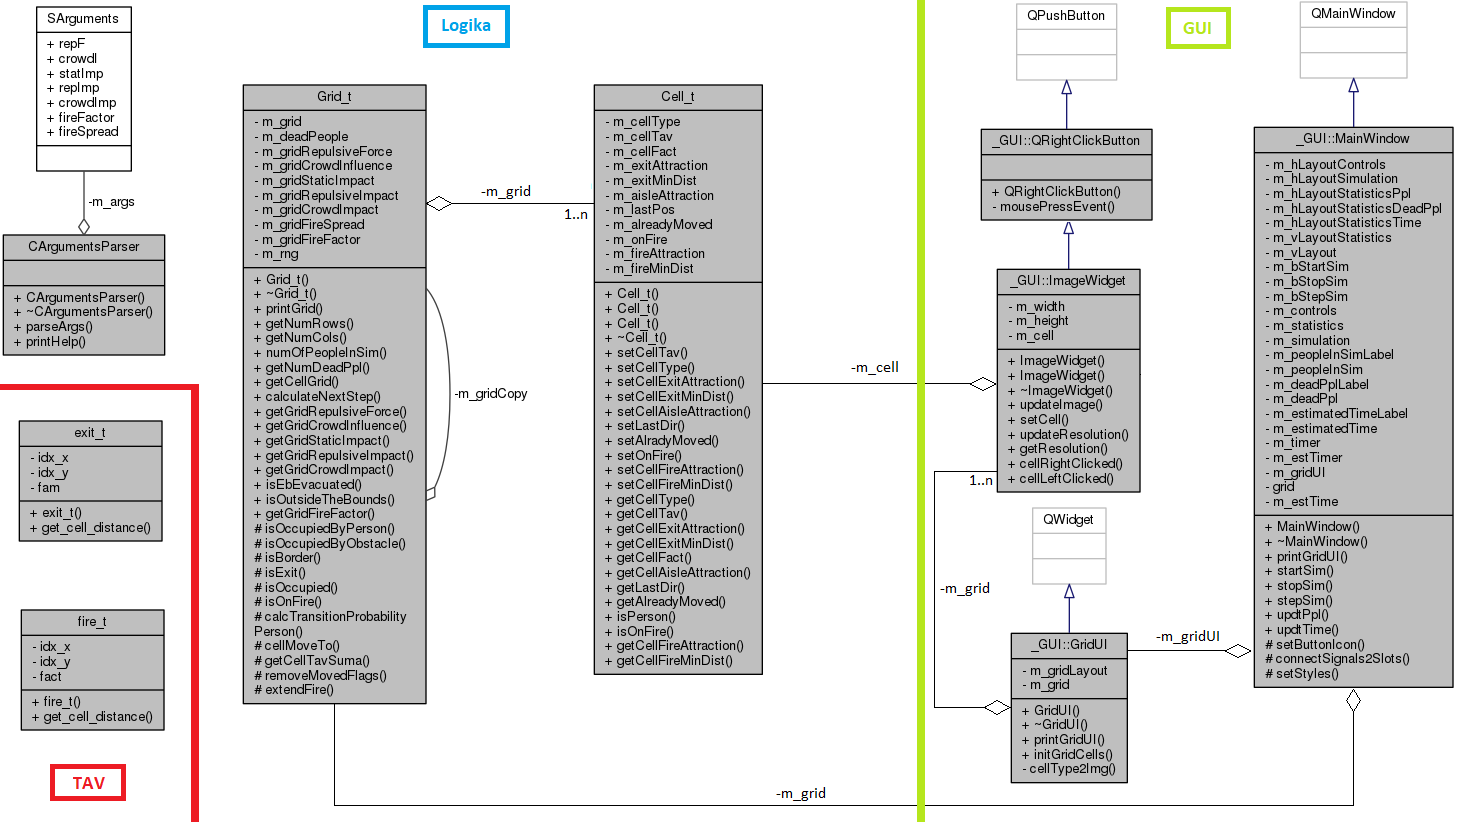
\includegraphics[scale=0.45]{class_diagram.png}
    
    V~diagramu jasně vidíme tři hlavní části aplikace. Část TAV, jež zajišťuje výpočet atraktivity buněk. Část GUI, která zajišťuje vizualizaci a částečnou kontrolu simulace. Poslední, ale neméně důležitá část je Logika zajišťující výpočet pravděpodobností, zpracování argumentů a celkovou logiku aplikace. 

\section{Architektura simulačního modelu/simulátoru} \label{sec:implementation}
    Program je členěn do následujících modulů obstarávající jednotlivé úkony v~systému.
    
    Pro simulaci nepodstatný modul Args zpracovávající argumenty příkazové řádky.
    
    Jak už z~názvu celulární vyplývá, buňky jsou v~simulaci základním stavebním kamenem. Tyto buňky jsou reprezentovány instancemi třídy Cell\_t, jež se nachází v~modulu Cell. Buňka udržuje informaci o~tom, jakého je typu (tedy člověk, překážka, ...), dále obsahuje stavovou proměnnou s~informací o~tom, zda buňka hoří, směr posledního pohybu a~hodnoty potřebné pro výpočet TAV.
    
    Tyto buňky jsou sdružovány do 2D pole reprezentující prostor simulovaného prostředí (v~našem případě kino-sál). Takovýto prostor je implementován v~modulu s~názvem Grid. Grid zastupuje podstatnou roli po dobu celé simulace. Obsahuje zapouzdřené hlavní proměnné celé simulace a~provádí nad nimi jednotlivé operace v~daném pořadí. Pro případy, kdy je při výpočtu potřeba provést více kroků pro stejné rozložení a~hodnoty buněk (např. při výpočtu TAV a pravděpodobností pro přesun lidí) obsahuje Grid kopii sebe sama.
    
    Poslední, ale neméně důležitý modul TAV obsahuje výpočet tzv. total attraction value, potřebnou pro výpočet pravděpodobností pro přechod na jednotlivé sousední buňky. \\
    
    Tento odstavec detailně popisuje pseudokód Algorithm \ref{alg:alg1}. Simulace začíná zpracováním vstupních argumentů příkazové řádky, které se poté předají konstruktoru třídy \texttt{Grid\_t}. Pokud je nastaven vstupní příznak pro založení ohně, je vygenerována náhodná pozice v~rámci pole buněk~a tam umístěno ohniště. Poté se vstoupí do smyčky, která skončí až poté, co jsou všichni lidé evakuováni, potažmo zemřou. V~rámci cyklu se provádí jednotlivé kroky simulace pomocí metody třídy \texttt{Grid\_t}, nazvané \texttt{calculateNextStep()}. Poté se aktualizují statistiky, v~případě vizuálního módu se překreslí pole buněk, vlákno se uspí na určitou krátkou dobu, a~pokračuje se v~cyklu. V~případě, že řízení programu vystoupí ze smyčky, tedy všichni lidé opustí simulaci, vypíší se na standardní výstup či do GUI statistiky a~simulace končí.
    
    Tento odstavec detailně popisuje pseudokód Algorithm \ref{alg:alg2}. V~rámci metody \texttt{calculateNextStep()}, volané z~hlavní smyčky, se vytvoří kopie celého pole buněk, a~postupně se prochází jednotlivé buňky. Protože pro případy, kdy se začínalo pole buněk procházet zleva, měli lidé v~simulaci tendenci jít spíše doleva (podobně pro začátek procházení zprava), se vyhodnocují buňky náhodně -- tzn. že vektor všech souřadnic se před každým procházením "zamíchá". Pro každou buňku se volá metoda \texttt{extendFire()}, která zjišťuje šanci na vzplanutí této buňky a na základě pseudo-náhodně vygenerovaného čísla může tuto buňku zapálit. Pokud buňka reprezentuje člověka a~zároveň není nastavený příznak, že se tento člověk už v~rámci tohoto kroku pohnul, volá se zapouzdřená metoda pro výpočet pravděpodobností pro tohoto člověka. Příznak, zda se osoba už v~rámci kroku pohnula, se na konci každého simulačního kroku nuluje u~všech osob v~simulaci. Při výpočtu pravděpodobností pro jednotlivé směry chůze je třeba projít osmi-okolí této buňky a~pro každou, která je prázdná (není tam stěna, člověk ani překážka) se počítá pravděpodobnost pohybu osoby na tuto buňku. Poté co se takto projde celé pole buněk, se resetují již zmíněné příznaky, zda se osoba už pohnula, zdestruuje se kopie pole buněk a řízení programu se vrací do smyčky, odkud byla metoda volána.
    
    Tento odstavec detailně popisuje pseudokód Algorithm \ref{alg:alg3}. Při výpočtu pravděpodobností pro sousední buňky osoby z~osmi-okolí se počítá se vzorcem pro výpočet pravděpodobnosti \ref{eq_Pij}. Poté co jsou pomocí tohoto vzorce vypočítány pravděpodobnosti, je vygenerováno pseudo-náhodné číslo na základě uniformního rozložení. Na základě tohoto čísla se vybere další krok (v~závislosti na pravděpodobnostech) a~člověk se přesune na určenou pozici. Tento přesun se ovšem neděje v~rámci kopie pole buněk, nýbrž v~originálním poli buněk. Poté se uloží informace o~směru posledního pohybu člověka pro další výpočty a pokračuje se další buňkou.
    
    
    \subsection{Generování pseudo-náhodných čísel}
    Pro generování pseudo-náhodných čísel jsme využili generátor 32-bitových celých čísel s~uniformním rozdělením, založený na algoritmu Mersenne Twister implementovaný ve standardu C++11.

    \subsection{Grafické uživatelské rozhraní}
    Simulaci jsme doplnili o vizualizaci a kontrolu simulace pomocí grafického uživatelského rozhraní, jenž diskrétně (každý krok) zobrazuje aktuální stav systému. Umožňuje dynamicky měnit stav systému pomocí změny typu jednotlivých buněk. Mimo to umožňuje kontrolu průběhu simulace a zobrazuje aktuální statistiky. Uživatelské rozhraní je implementováno v~jazyce C++ za pomoci frameworku Qt kvůli přenositelnosti.
    
    GUI se skládá ze třech částí. 1) Tlačítka pro řízení simulace, 2) Statistiky a 3) Zobrazení 2D prostoru.
    
    Tlačítka jsou tři. Pomocí zeleného tlačítka lze začít simulaci -- spustí se čas a lidé se začnou hýbat. Provádí se jednotlivé kroky s~určitou dobou spánku mezi kroky až do doby, kdy je simulace dokončena (všichni lidé opustí prostor nebo zemřou) nebo zastavení simulace. Zastavení simulace lze docílit zmáčknutím červeného tlačítka, které zastaví jak čas, tak pohyb lidí. Třetí a poslední modré tlačítko slouží pro provedení jednoho kroku simulace.
    
    Statistiky zobrazují uplynulý čas od počátku simulace, počet lidí, kteří stále neopustili simulovaný prostor a počet lidí, kteří zahynuli od počátku simulace.
    
    Nejdůležitější část GUI, vizualizující simulovaný prostor, se skládá z~tlačítek. Každá buňka je reprezentována právě jedním tlačítkem. Levým kliknutím myši lze přidat/odebrat východ. Podobně pravým tlačítkem myši lze přidat/odebrat ohnisko.
    
    \subsection{Sestavení a spuštění}
    Aplikaci je možné sestavit ve třech různých módech.
    Nejdůležitější pro simulaci je verze s~GUI, kterou lze sestavit pomocí \texttt{make gui}. Jak už je zmíněno výše, tato verze je závislá na knihovně Qt.
    
    Poté je konzolová verze, jenž se sestaví pomocí \texttt{make} a statistiky i průběh simulace vypisuje na standardní výstup. Poslední -- ladící verze, která na standardní výstup píše log o všem, co provádí. Tato verze se sestavuje pomocí \texttt{make debug}.
    
    Všechny verze v~hlavním adresáři vytvoří spustitelný soubor \texttt{IMS\_xkocic01\_xvasic25(\_gui)} který lze spustit bez parametrů (jsou použity výchozí parametry simulace) nebo jej lze konfigurovat pomocí příkazové řádky, viz přepínač -h.

    \subsection{Mapování konceptuálního modelu do simulačního modelu}
    Jednotlivé buňky simulačního prostoru jsou implementovány třídou Cell\_t poskytující rozhraní pro získávání a nastavování hodnot buňky. Dvou-rozměrné pole těchto buněk je obsaženo v~třídě Grid\_t, jenž reprezentuje celý simulační prostor (kino-sál). Vzorec pro výběr směru pohybu osoby (vzorec č.\ref{eq_Pij}) je implementován v~metodě gridu \texttt{calcTransitionProbabilityPerson()}. Funkce pro výpočet atraktivity (vzorec č.\ref{eq_Nij}) je implementována ve funkci \texttt{get\_cell\_tav()} v~modulu TAV.

\section{Podstata simulačních experimentů a jejich průběhu}
\label{experiments}
Celkovým cílem této studie je nalézt optimální množství a~rozložení východů z~místnosti modelující kino-sál. Metrikou pro porovnání jednotlivých rozložení je celkový čas evakuace. Provádět takové experimenty fyzicky by bylo náročné z~časového i~zdrojového hlediska. Simulační model tedy umožní experimentů provést mnohem více a~navíc bez nutnosti budovat fyzický model místnosti. Provedli jsme tři kategorie experimentů. První kategorie experimentů sloužila pro testování a~validaci modelu. Jejich cílem není dosáhnout minimálního času evakuace, ale pozorovat chování jednotlivých buněk v~různých situacích a~s~různými simulačními parametry. Druhá kategorie tvoří největší část experimentů a~je zaměřena na hledání minimálního času evakuace bez přítomnosti ohně. Pro tyto experimenty je jedinou metrikou celkový čas evakuace. Poslední kategorií jsou testy obsahující šířící se oheň. Jejich úkolem je nalézt taková rozložení východů, která minimalizují úmrtí osob. Čas evakuace v~těchto testech hraje sekundární roli (delší evakuace ale znamená větší rozšíření ohně).


    \subsection{Postup experimentování}
    Experimenty byly prováděny pomocí verze simulátoru s~grafickým uživatelským rozhraním, především protože umožňuje snadno upravovat výchozí stav simulace. Rozložení východů lze dokonce měnit za běhu, toto ale slouží především pro ulehčení testování. Postup testovacích experimentů není jednotně definovatelný. Obecně byl spuštěn simulační nástroj a~s~případnými úpravami rozložení místnosti spuštěna nebo krokována simulace. Zbylé "řádné" experimenty probíhaly všechny stejně. Po spuštění simulátoru je definováno rozložení východů a~spuštěna simulace. Po skončení simulace je zaznamenán celkový čas a~pro experimenty s~přítomností ohně i~počet mrtvých osob.

    \subsection{Testovací experimenty}
    \label{test_experiments}
    Sekce s~experimenty zaměřenými na testování simulátoru a~jeho validity. Podstatou je sledovat chování buněk za různých podmínek a~různých simulačních parametrů. Testovacích experimentů bylo provedeno daleko více, než je zde uvedeno, ne všechny ale byly dokumentovány.

        \subsubsection{Pohyb osob bez východů nebo ohně}
        Experiment ukazuje pohyb osob po místnosti bez cíle. Používá výchozí parametry simulace. Obrázek~\ref{noExit_noFire} zobrazuje počáteční stav (vlevo) a stav po 50s simulace. Osoby jsou rozprostřeny poměrně rovnoměrně po místnosti, jak bylo očekáváno, když nemají žádný cíl. Lze pozorovat atraktivitu hlavních uliček, ve kterých se nachází většina osob.\\

        \begin{figure}[H]
            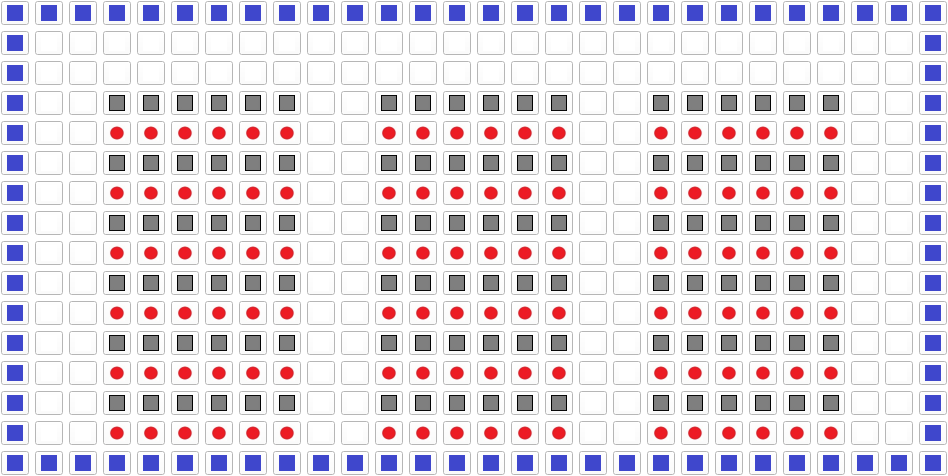
\includegraphics[width=8cm]{gui_initial_state}
            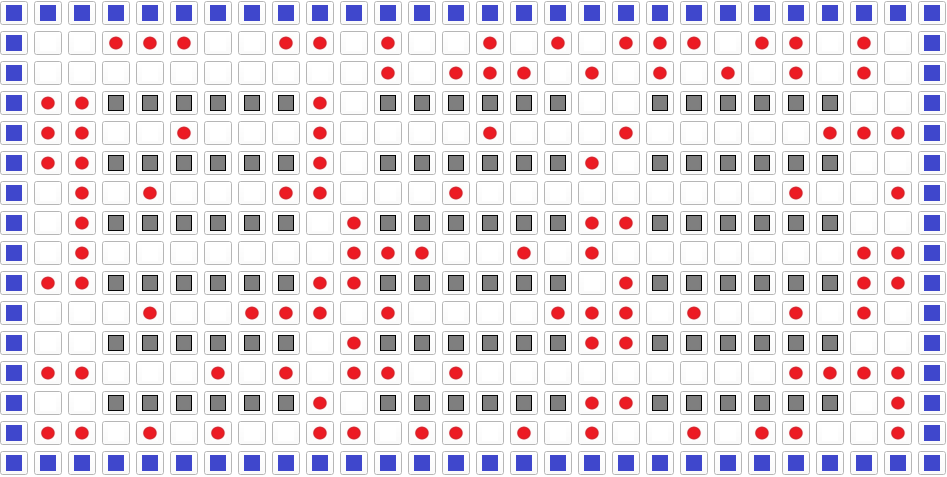
\includegraphics[width=8cm]{TestLayouts/noExit_noFire}
            \caption{Pohyb osob bez východů nebo ohně}
            \label{noExit_noFire}
        \end{figure}

        \subsubsection{Pohyb osob s~jedním východem }
        Experiment ukazuje pohyb osob po místnosti s~jedním východem. Používá výchozí parametry simulace. Obrázek~\ref{oneExit_noFire} zobrazuje počáteční stav (vlevo) a~stav po asi 30s simulace. Lze pozorovat, že všechny osoby směřují k~východu.\\

        \begin{figure}[H]
            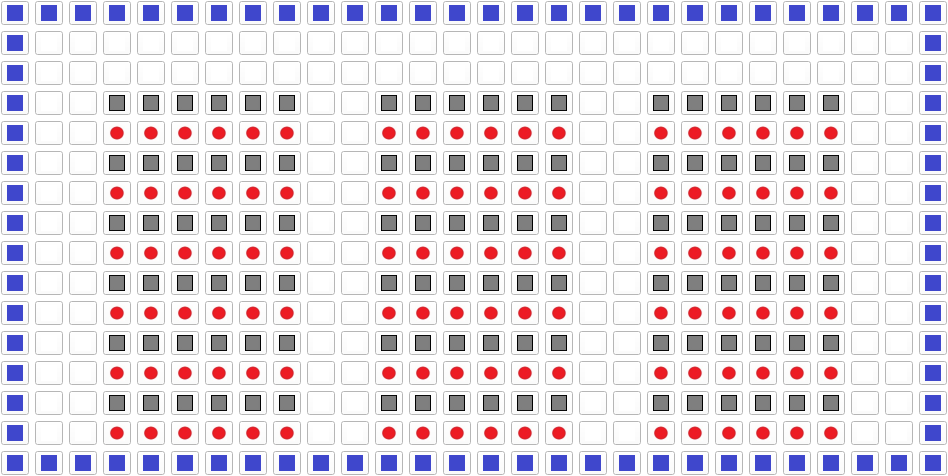
\includegraphics[width=8cm]{gui_initial_state}
            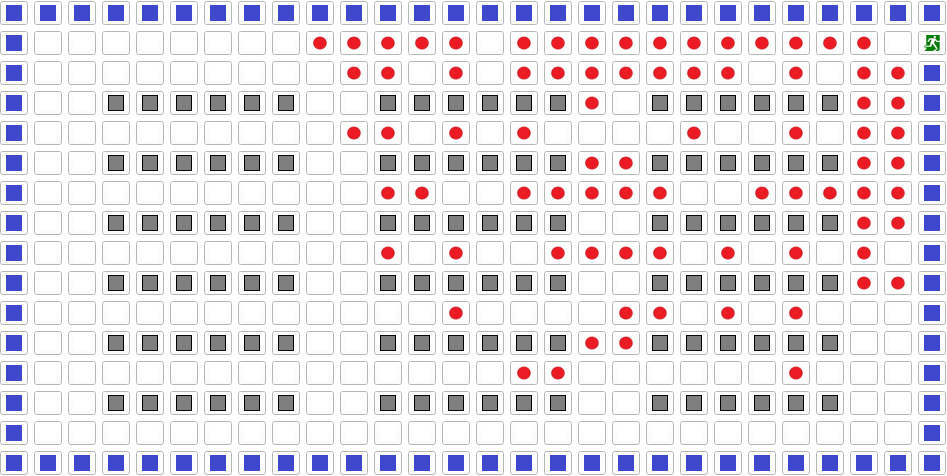
\includegraphics[width=8cm]{TestLayouts/oneExit_noFire}
            \caption{Pohyb osob s~jedním východem}
            \label{oneExit_noFire}
        \end{figure}

        \subsubsection{Pohyb osob s~více východy}
        Experiment ukazuje pohyb osob po místnosti s~více východy. Používá výchozí parametry simulace. Obrázek~\ref{twoExits_noFire} zobrazuje počáteční stav (vlevo) a~stav po asi 20s simulace. Lze pozorovat, že osoby směřují k~oběma východům přibližně rovnoměrně.\\

        \begin{figure}[H]
            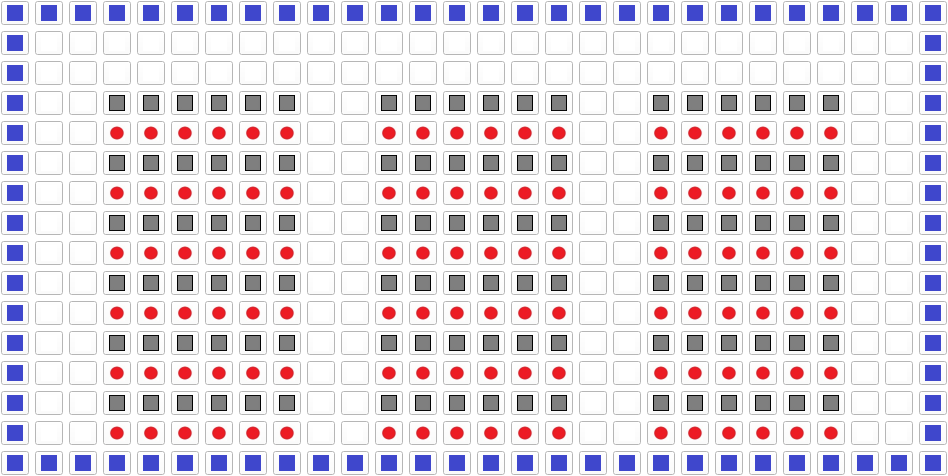
\includegraphics[width=8cm]{gui_initial_state}
            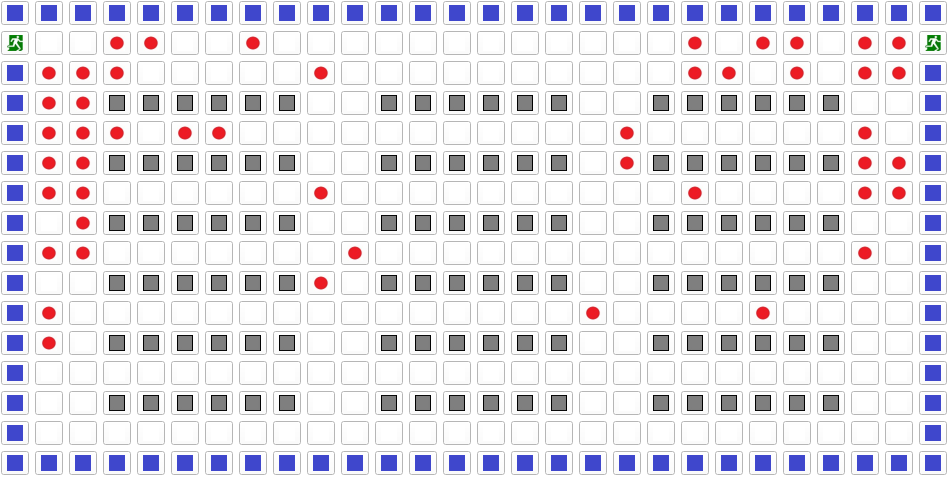
\includegraphics[width=8cm]{TestLayouts/twoExits_noFire}
            \caption{Pohyb osob s~více východy}
            \label{twoExits_noFire}
        \end{figure}


        \subsubsection{Pohyb osob a šíření ohně bez východů}
        Experiment ukazuje pohyb osob po místnosti bez východů s přítomností ohně. Používá výchozí parametry simulace. Obrázek~\ref{noExit_oneFire} zobrazuje počáteční stav (vlevo) a stav po asi 30s simulace. Lze pozorovat, že osoby se snaží vzdalovat od ohně. Šíření ohně je také poměrně rovnoměrné.\\

        \begin{figure}[H]
            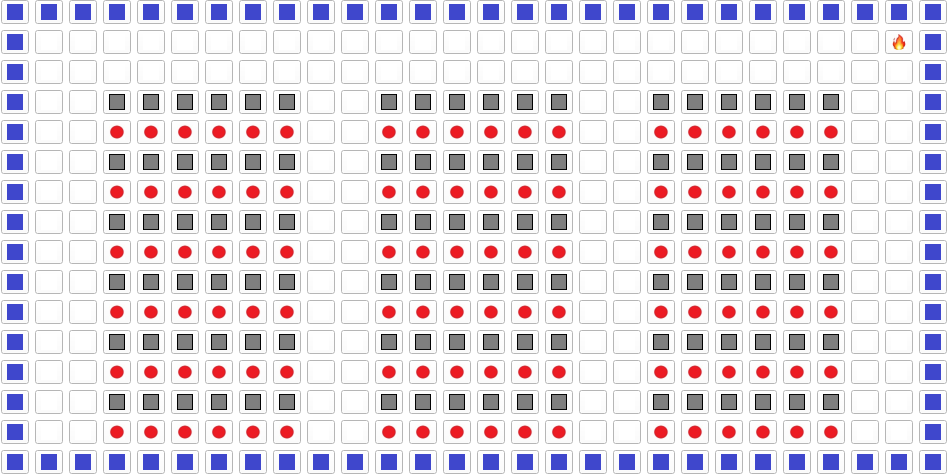
\includegraphics[width=8cm]{TestLayouts/fire_initial_state}
            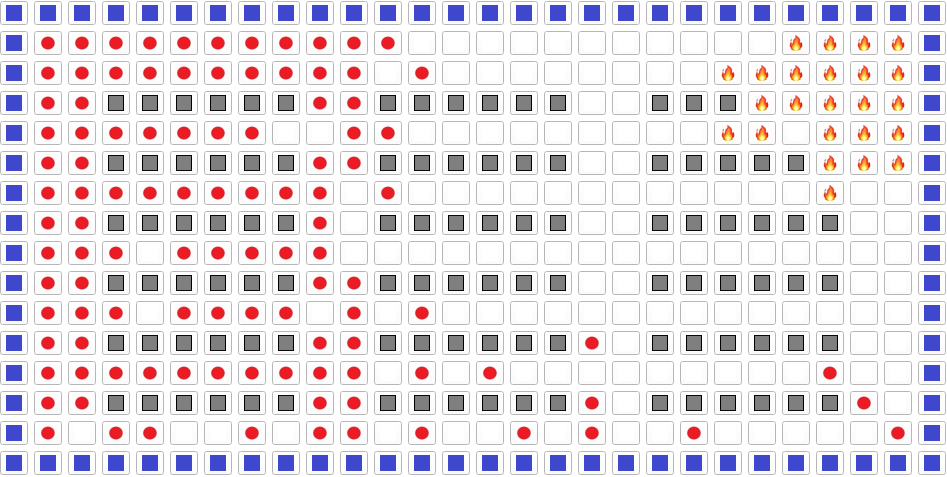
\includegraphics[width=8cm]{TestLayouts/noExit_oneFire}
            \caption{Pohyb osob a šíření ohně bez východů}
            \label{noExit_oneFire}
        \end{figure}

        \subsubsection{Pohyb osob s~ohněm a východem na stejné straně místnosti}
        \label{exp_onefire_oneexit}
        Experiment ukazuje pohyb osob po místnosti s~jedním východem a~ohněm na stejné straně. Oheň je tedy poměrně blízko východu. Experiment používá výchozí parametry simulace. Do místnosti je nejdříve přidán oheň. Po přesunu osob na opačnou stranu místnosti je přidán východ na stranu shodnou ohni. Obrázek~\ref{FireExitSameSide} zobrazuje osoby utíkající od ohně a zbytek osob směřujících k~východu po jeho přidání asi po 100s simulace. Osoby tedy směřují k~východům i přes nutnost přiblížit se ohni, evakuace ale trvá výrazně déle.\\

        \begin{figure}[H]
            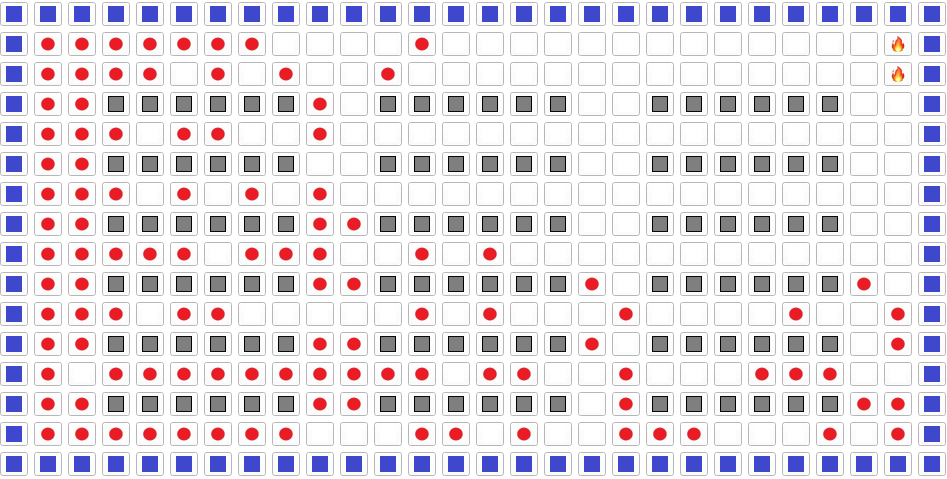
\includegraphics[width=8cm]{TestLayouts/FireExitSameSide/FireExit_SameSide_init}
            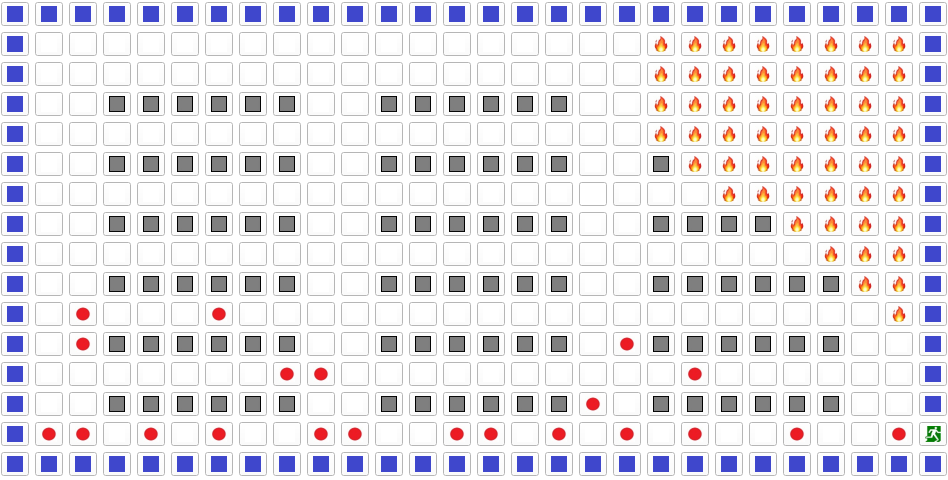
\includegraphics[width=8cm]{TestLayouts/FireExitSameSide/FireExit_SameSide_ExitAdded}
            \caption{Pohyb osob s~ohněm a východem na stejné straně místnosti}
            \label{FireExitSameSide}
        \end{figure}


        \subsubsection{Odhalení dopadu sekvenčního procházení pole buněk na symetrii pohybu}
        Pole buněk bylo původně procházeno během výpočtu pohybu osob sekvenčně podle rostoucích indexů. Tento postup ale přinášel do simulace nesymetričnost. Obrázek~\ref{indexBug} vlevo zobrazuje stav simulace po provedení dvou až čtyř kroků. Lze jasně pozorovat, že první tři vertikální uličky zleva jsou plné osob, zatímco čtvrtá ulička je téměř prázdná. Indexování vždy zleva způsobuje, že osoby více vlevo se pohnout dříve a uvolní tak místo osobě od nich vpravo. Všechny osoby v~řadě sedadel se tak mohou pohnout doleva v~jednom kroku simulace. Pravá část obrázku zobrazuje stejnou situaci po zavedení náhodného indexování a lze pozorovat, že všechny vertikální uličky jsou přibližně stejně obsazené.\\

        \begin{figure}[H]
            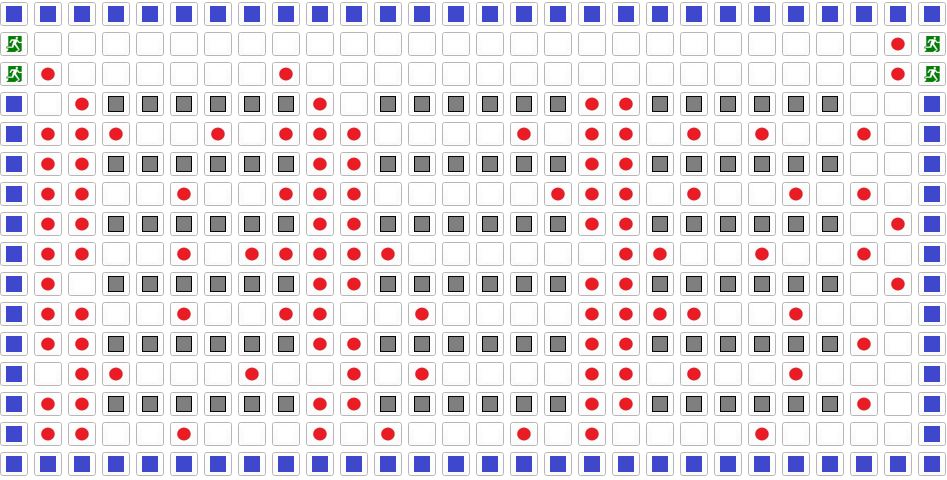
\includegraphics[width=8cm]{BugFixes/index_seq_bug}
            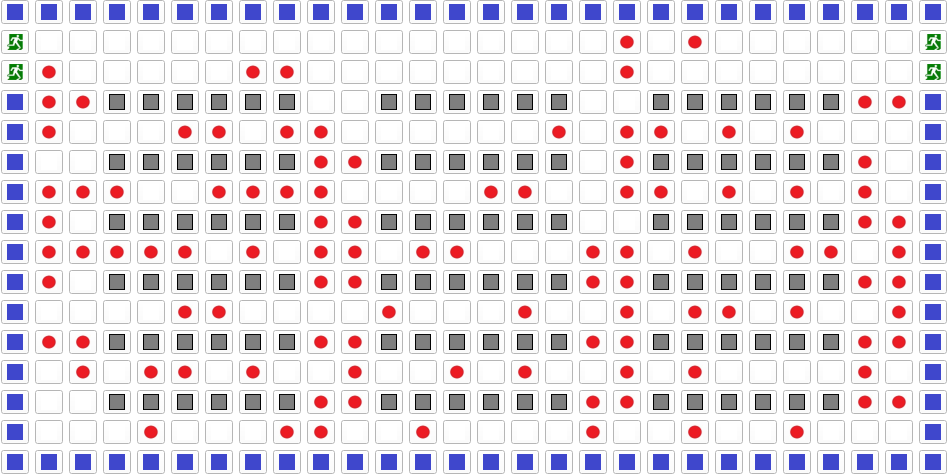
\includegraphics[width=8cm]{BugFixes/index_seq_bug_fixed}
            \caption{Nesymetričnost způsobená sekvenčním indexováním}
            \label{indexBug}
        \end{figure}

        \subsubsection{Pozorování vlivu atraktivity uliček}
        Experiment ukazuje pohyb osob po místnosti bez východu s~použitím parametru atraktivity s~hodnotou $5.0$ oproti hodnotě $0.0$. Ostatní parametry simulace zůstávají výchozí. Obrázek~\ref{testAisle} zobrazuje vlevo simulaci s~vysokým vlivem uliček a vpravo simulaci bez vlivu uliček. Při použití vysoké hodnoty parametru je většina osob v~uličkách a bez něj jsou osoby rozloženy rovnoměrně po celé místnosti.\\

        \begin{figure}[H]
            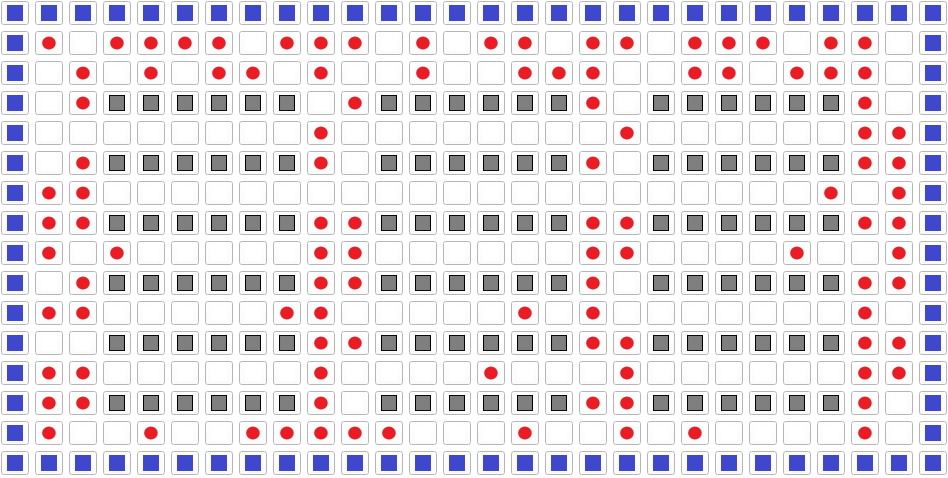
\includegraphics[width=8cm]{TestParams/highAisle}
            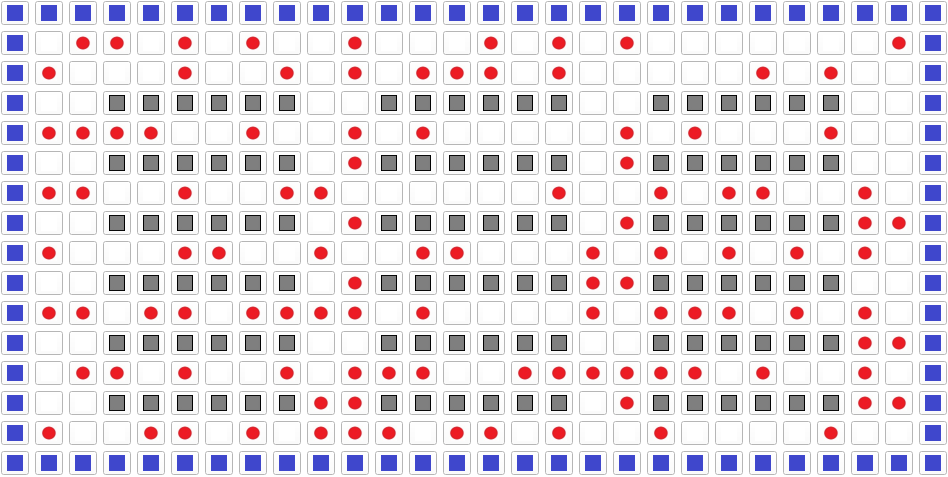
\includegraphics[width=8cm]{TestParams/noAisle}
            \caption{Demonstrace vlivu atraktivity hlavních uliček}
            \label{testAisle}
        \end{figure}

        \subsubsection{Pozorování vlivu odpudivé síly mezi lidmi}
        Experiment ukazuje pohyb osob po místnosti s~jedním východem s~použitím vlivu odpudivé sily s~hodnotou $5.0$ oproti hodnotě $0.0$. Ostatní parametry simulace zůstávají výchozí. Obrázek~\ref{testRep} zobrazuje vlevo simulaci s~velkým vlivem odpudivé síly a vpravo simulaci bez vlivu odpudivé síly. Bez použití odpudivé síly se lidé výrazně více mačkají na sebe. Vniká tak u~východu větší jednolitý obdélník buněk s~osobami.\\

        \begin{figure}[H]
            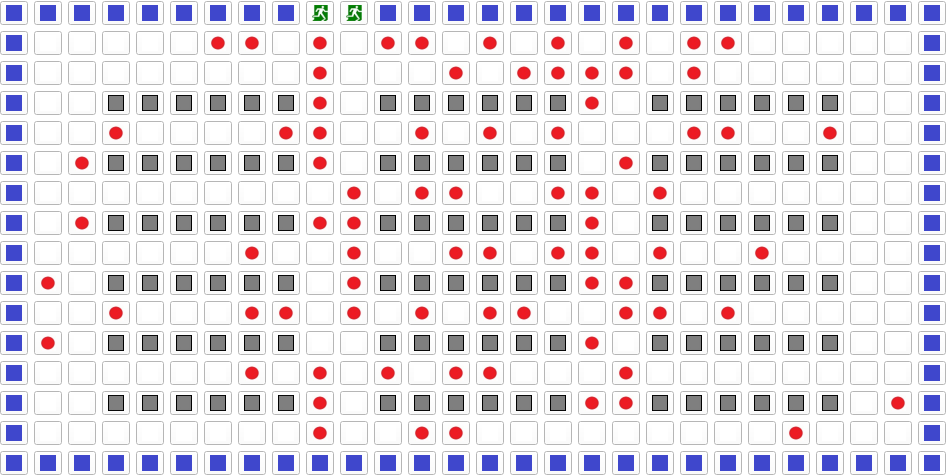
\includegraphics[width=8cm]{TestParams/highRep}
            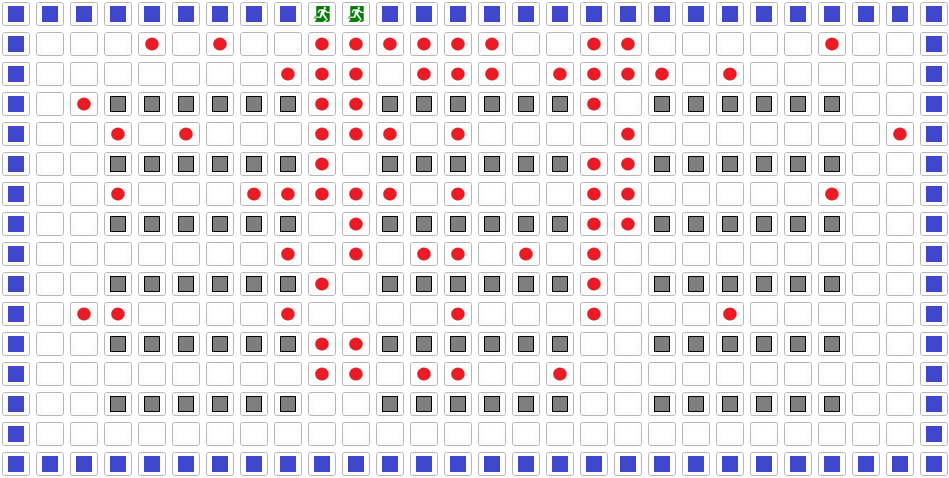
\includegraphics[width=8cm]{TestParams/noRep}
            \caption{Demonstrace vlivu odpudivé síly mezi lidmi}
            \label{testRep}
        \end{figure}

        \subsubsection{Pozorování vlivu následování davu}
        Experiment ukazuje pohyb osob po místnosti v~situaci obdobné jako v~experimentu~\ref{exp_onefire_oneexit} s~použitím vlivu následování davu s~hodnotou $5.0$ oproti hodnotě $0.0$. Rozsah dohledu osob byl zvýšen na $10$. Ostatní parametry simulace zůstávají výchozí. Obrázek~\ref{testCrow} zobrazuje vlevo simulaci s~velkým vlivem následování davu a vpravo simulaci bez vlivu následování davu. V~důsledku toho, že většina osob přešlapuje sem a tam v~pravém dolním rohu a jen malá část osob postupuje k~východu po horním okraji, je tendence pohybu davu proměnná do všech směrů a pro osoby je v~dané situaci přítěží. V~simulaci bez vlivu davu došlo k~evakuaci většího množství osob během shodného rozšíření ohně.\\

        \begin{figure}[H]
            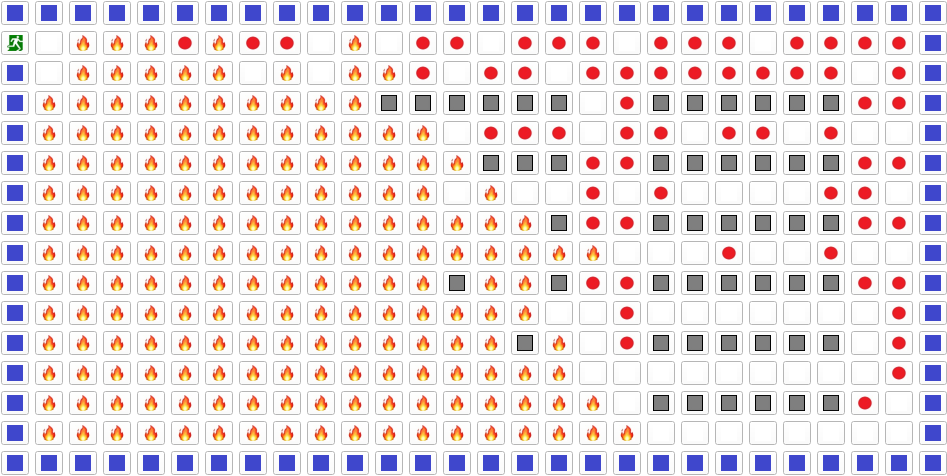
\includegraphics[width=8cm]{TestParams/highCrow}
            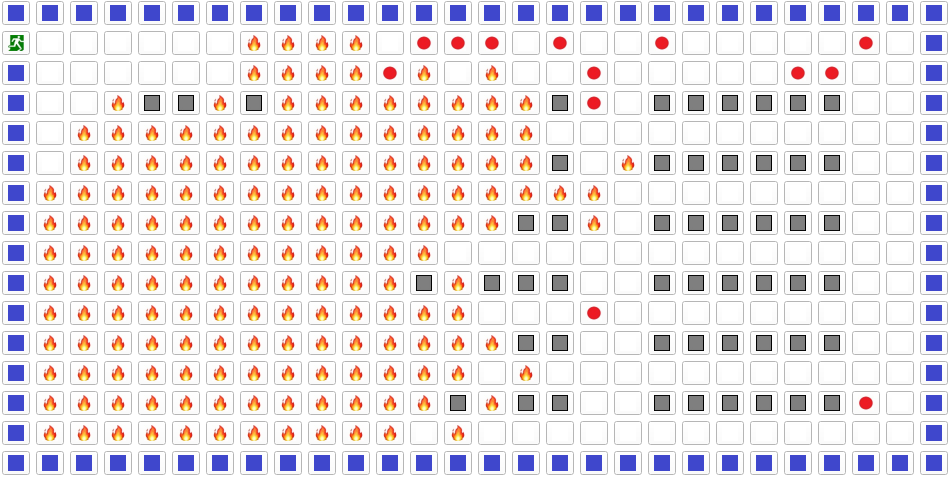
\includegraphics[width=8cm]{TestParams/noCrow}
            \caption{Demonstrace vlivu následování davu}
            \label{testCrow}
        \end{figure}


        \subsubsection{Experiment s~lidmi s~fobií z~ohně}
        Experiment ukazuje pohyb osob po místnosti v~situaci obdobné jako v~experimentu~\ref{exp_onefire_oneexit} s~použitím hodnoty odpudivé síly ohně o velikosti $5.0$ oproti hodnotě $0.0$. Ostatní parametry simulace zůstávají výchozí. Obrázek~\ref{testFire} vlevo ukazuje simulaci s~použitím vysoké odpudivé síly davu - místnost neopustila ani jedna osoba. V~pravé části je simulace bez odpudivé síly ohně, ve které simulaci opustilo 70\% osob a zbytek uhořel, protože osoby často beze strachu stály na buňce sousedící s~ohněm a riskovali tak vzplanutí.\\

        \begin{figure}[H]
            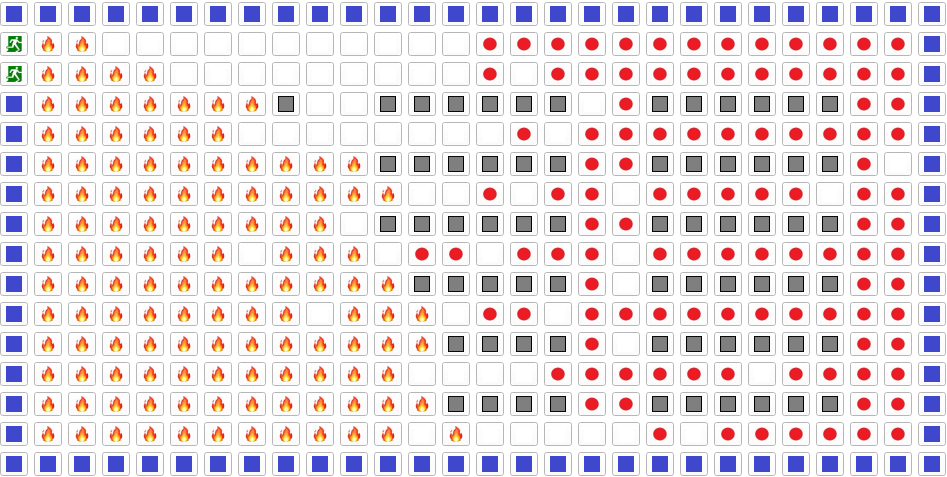
\includegraphics[width=8cm]{TestParams/highFire}
            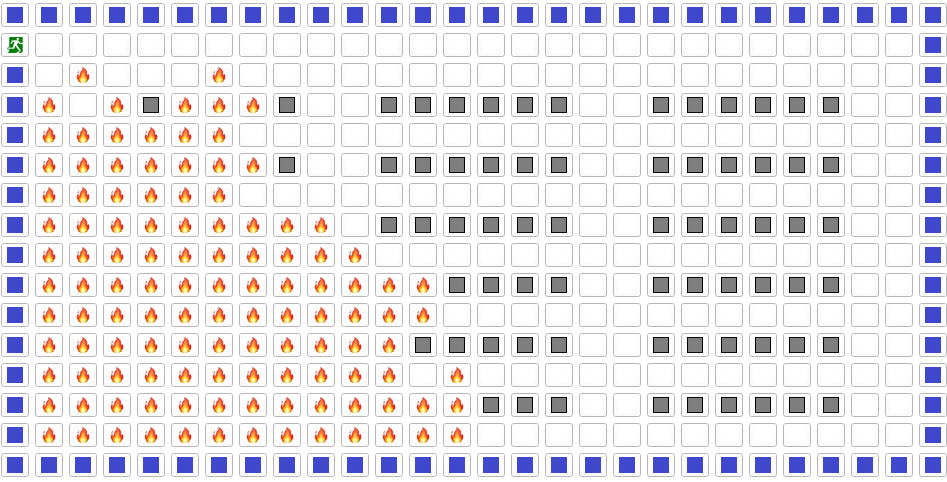
\includegraphics[width=8cm]{TestParams/noFire}
            \caption{Demonstrace vlivu odpudivé síly ohně}
            \label{testFire}
        \end{figure}


    \subsection{Hledání optimálního rozložení východů bez vlivu ohně}
    Tato sekce se zabývá hlavní myšlenkou této simulace a to optimálním rozložením a počtem východů. Dává smysl, že čím více východů v~simulovaném prostoru bude, tím rychleji se lidé evakuují. Je ovšem ale třeba počítat i s~náklady na výrobu východů a~konstrukčními omezeními. Proto je třeba najít optimální počet a~rozmístění východů experimenty.
    
        \subsubsection{Rozložení východů převzaté z~článku}
        Tento experiment je založen na rozložení východů uvedeném v~článku \textit{Cellular Automata Evacuation Model Considering Information Transfer in Building with Obstacles}~[1]. Jak lze vidět na obrázku \ref{testExits1}, evakuace s~tímto rozložením trvala v~průměru 48 sekund.
        
        \begin{figure}[H]
            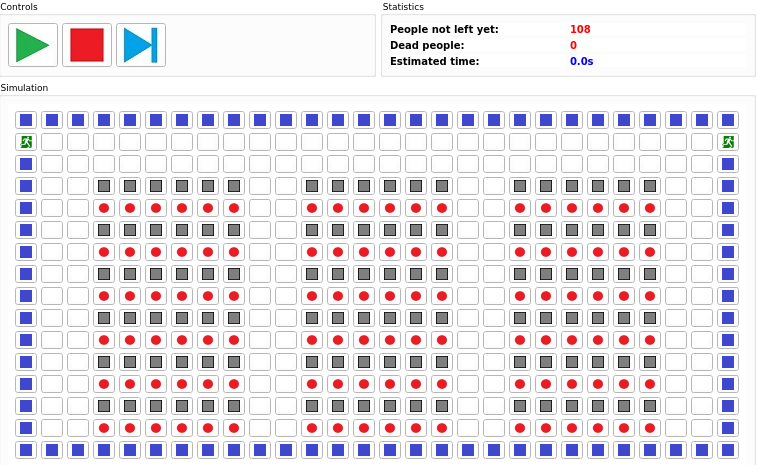
\includegraphics[width=8cm]{ExitDistribution/ExitsFromPaper}
            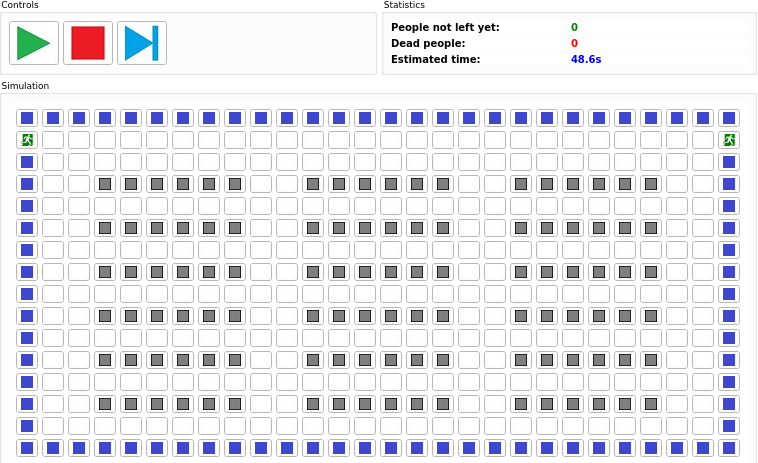
\includegraphics[width=8cm]{ExitDistribution/ExitsFromPaperEnd}
            \caption{Rozložení východů dle článku}
            \label{testExits1}
        \end{figure}
        
        \subsubsection{Druhý typ rozložení dvou východů} \label{exitDist2}
        Tento typ rozložení východů obsahuje východy uprostřed zdí simulovaného prostoru, tedy uprostřed řad kde sedí diváci v~kino-sále. Tento typ rozložení východů značně zrychlil evakuaci, viz obrázek \ref{testExits2}. Evakuace se oproti rozložení východů z~článku~[1] zrychlila v~průměru o 12 sekund, tedy čtvrtinu původního času.
        
        \begin{figure}[H]
            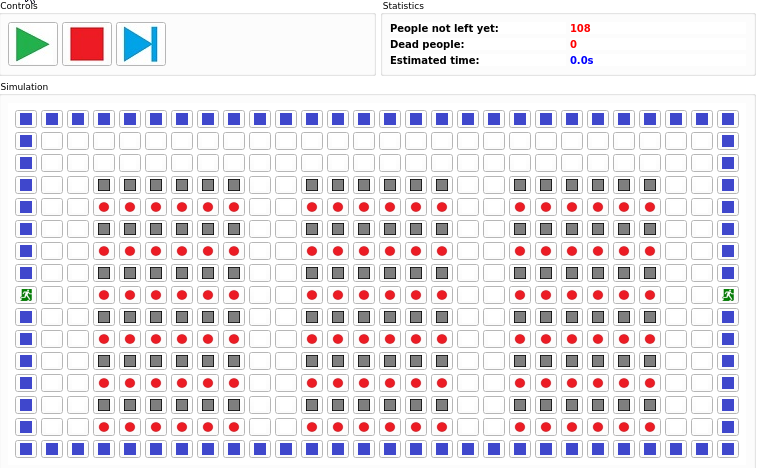
\includegraphics[width=8cm]{ExitDistribution/ExitDistribTwo}
            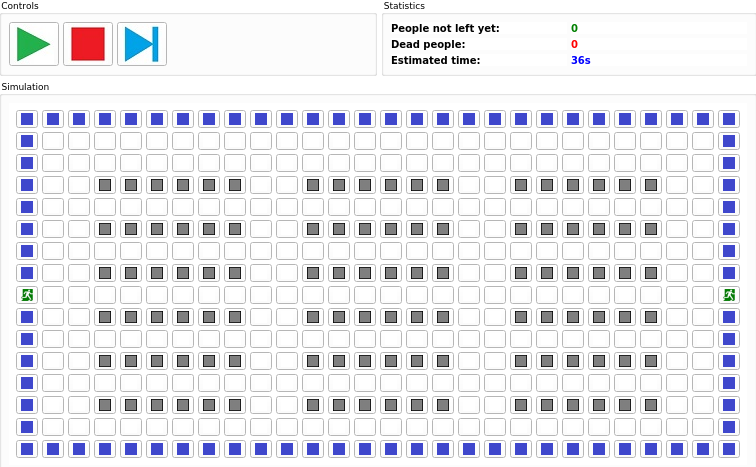
\includegraphics[width=8cm]{ExitDistribution/ExitDistribTwoEnd}
            \caption{Rozložení východů ve středu řad}
            \label{testExits2}
        \end{figure}
        
        \subsubsection{Třetí typ rozložení dvou východů}
        V~tomto pokuse jsme východy umístili do uliček mezi sloupci vzadu za diváky. Jak lze vidět na obrázku \ref{testExits3}, evakuace se oproti rozložení východů z~článku~[1] také výrazně zrychlila, nebyla ale natolik rychlá jako rozložení v~sekci \ref{exitDist2}.
        
        \begin{figure}[H]
            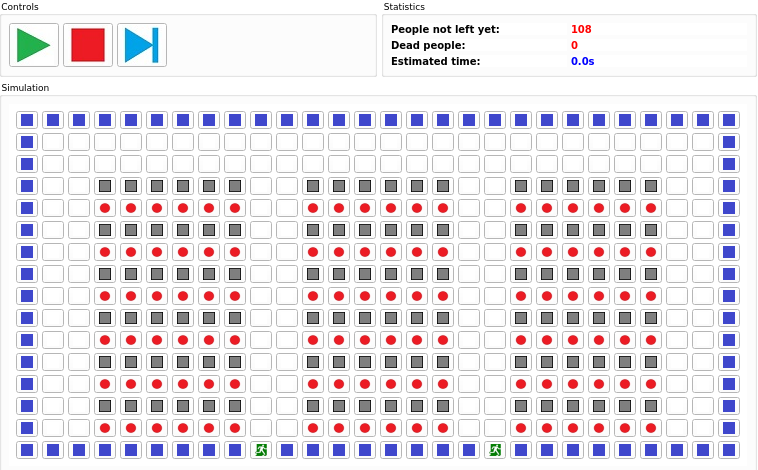
\includegraphics[width=8cm]{ExitDistribution/ExitDistribThree}
            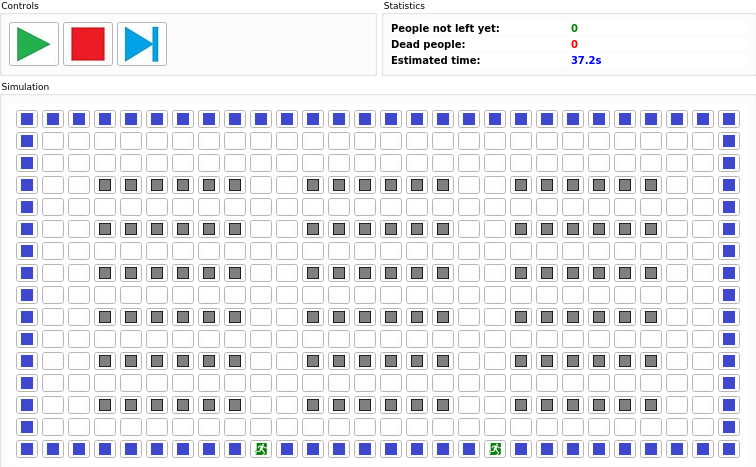
\includegraphics[width=8cm]{ExitDistribution/ExitDistribThreeEnd}
            \caption{Rozložení východů ve středu uliček}
            \label{testExits3}
        \end{figure}
        
        \subsubsection{První typ evakuace se třemi východy}
        Tento pokus do simulace přidává další východ. Toto rozložení je do jisté míry inspirováno rozložením z~článku~[1], avšak vzadu za diváky je přidán třetí východ, viz \ref{testExits4}. Tato simulace byla rychlejší než všechny simulace se dvěma východy, ale pouze o v~průměru dvě sekundy rychlejší, než nejrychlejší z~nich. Dle našeho úsudku tato doba nestojí za přidání dalšího východu.
        
        \begin{figure}[H]
            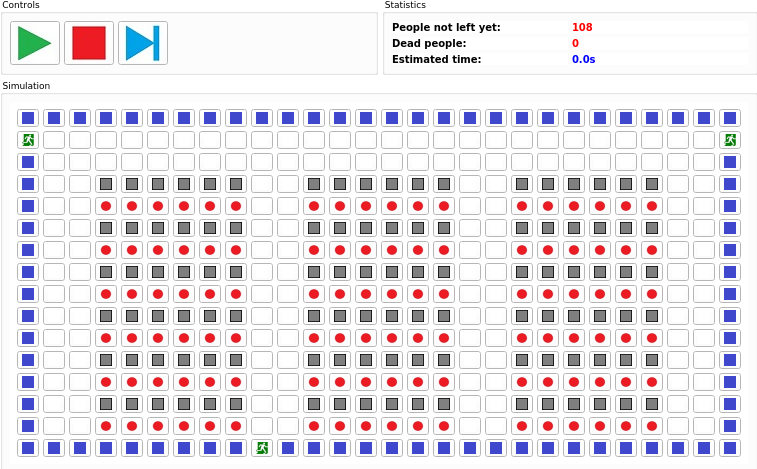
\includegraphics[width=8cm]{ExitDistribution/ExitDistribFour}
            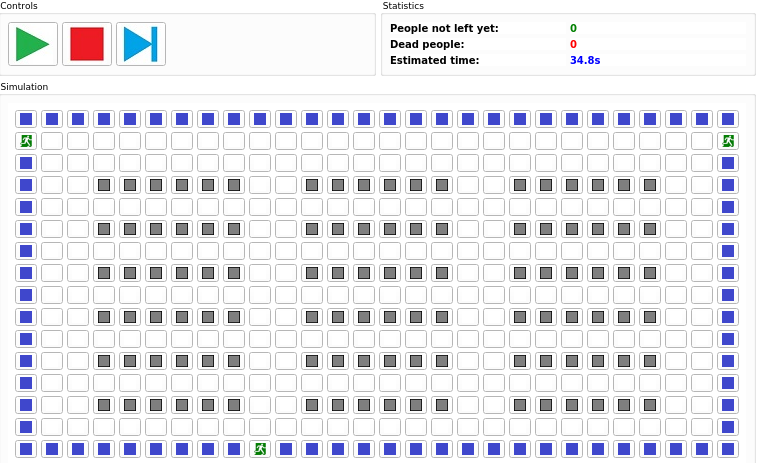
\includegraphics[width=8cm]{ExitDistribution/ExitDistribFourEnd}
            \caption{Rozložení východů se třemi východy inspirované článkem}
            \label{testExits4}
        \end{figure}
        
        \subsubsection{Druhý typ evakuace se třemi východy}
        V~tomto pokuse budeme používat rozložení východů z~nejlepšího rozložení východů se dvěma východy, doplněné o jeden další východ v~uličce. Dle očekávání má toto rozložení nejlepší výsledky, a to jak lze vidět na obrázku \ref{testExits5} je v~průměru 29 sekund. Přidání dalšího východu zde snížilo evakuaci o 7 vteřin, což už stojí za zvážení přidání dalšího východu.
        
        \begin{figure}[H]
            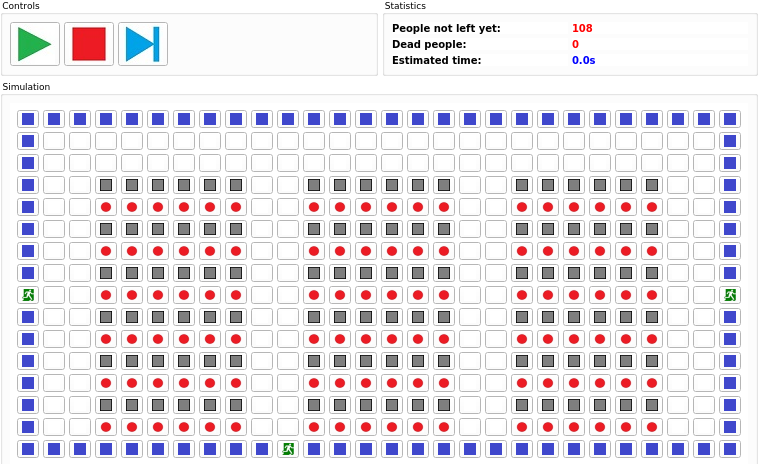
\includegraphics[width=8cm]{ExitDistribution/ExitDistribFive}
            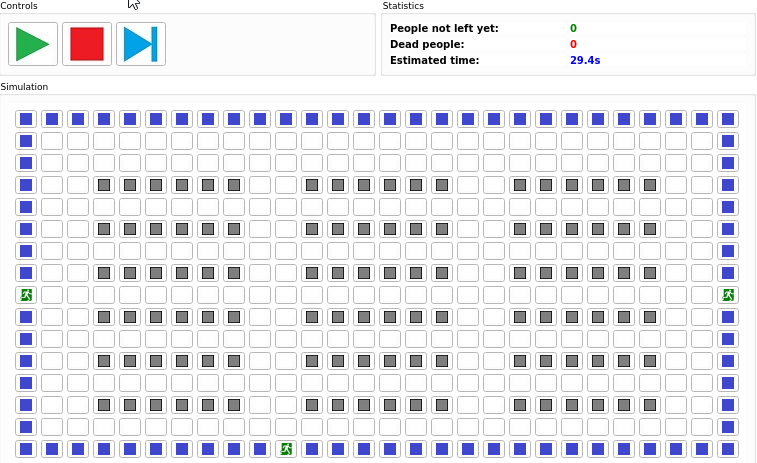
\includegraphics[width=8cm]{ExitDistribution/ExitDistribFiveEnd}
            \caption{Rozložení východů se třemi východy inspirované nejlepším rozložením dvou východů}
            \label{testExits5}
        \end{figure}
        
        \subsubsection{Evakuace se čtyřmi východy}
        Čtyři východy lze v~kino-sálech vidět jen velmi sporadicky. Rozložení východů bylo inspirováno nejlepším rozloženími východů dle předchozích experimentů, doplněné o jeden další východ. Jak lze vidět na obrázku \ref{testExits6}, se čtyřmi východy evakuace trvá v~průměru 30 sekund, což za přidání dalšího východu nestojí, protože již se třemi východy bylo dosaženo lepších výsledků, a to 29 sekund.
        
        \begin{figure}[H]
            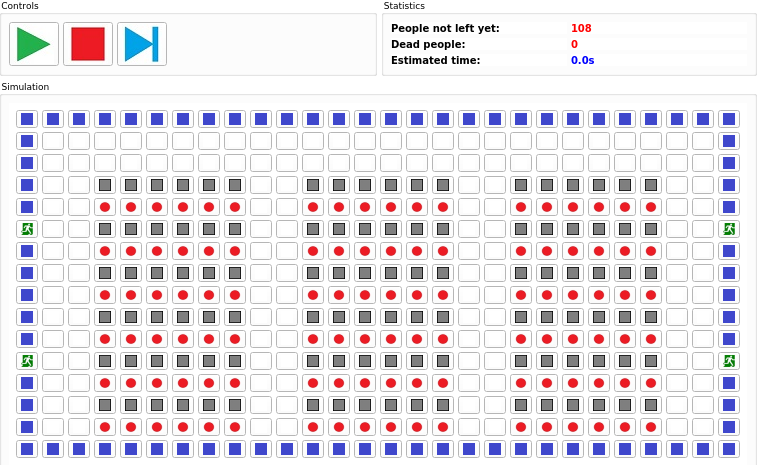
\includegraphics[width=8cm]{ExitDistribution/ExitDistribSix}
            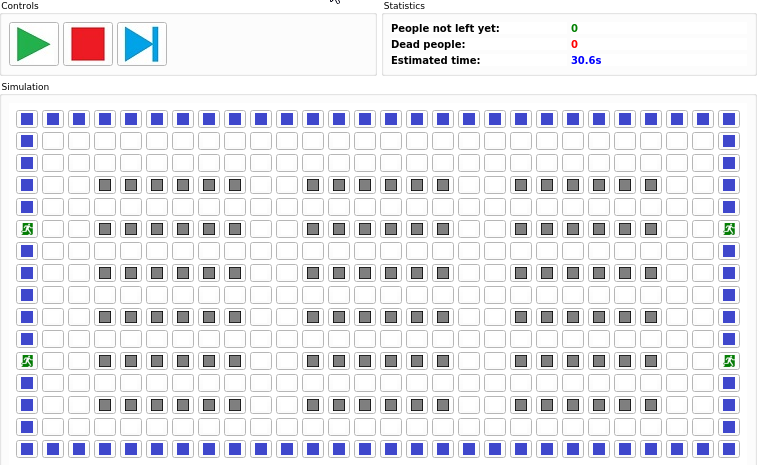
\includegraphics[width=8cm]{ExitDistribution/ExitDistribSixEnd}
            \caption{Rozložení východů se čtyřmi východy}
            \label{testExits6}
        \end{figure}
        
        \subsubsection{Evakuace se šesti východy}
        Nečekáme, že by někdo navrhl tak malý kino-sál se šesti východy, ale pro zajímavost přikládáme i tento experiment. Jak lze vidět na obrázku \ref{testExits7}, evakuace byla opravdu rychlá, a to v~průměru 17 sekund. Takto rychlá evakuace by ovšem měla velmi vysoké náklady a byla by aplikovatelná pouze ve výjimečných případech.
        
        \begin{figure}[H]
            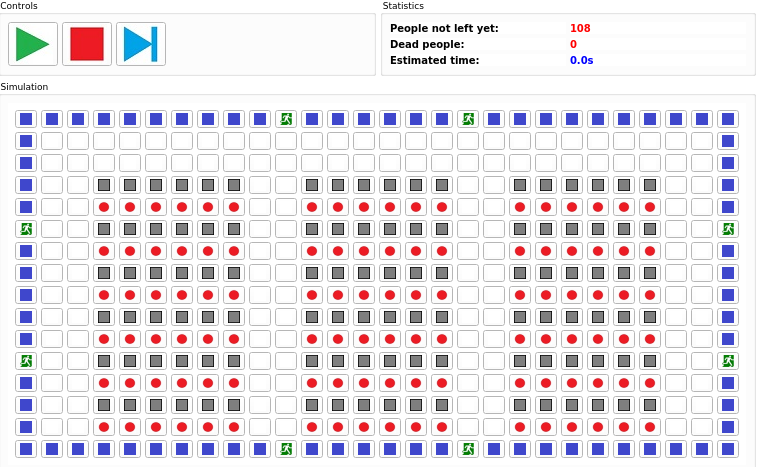
\includegraphics[width=8cm]{ExitDistribution/ExitDistribSeven}
            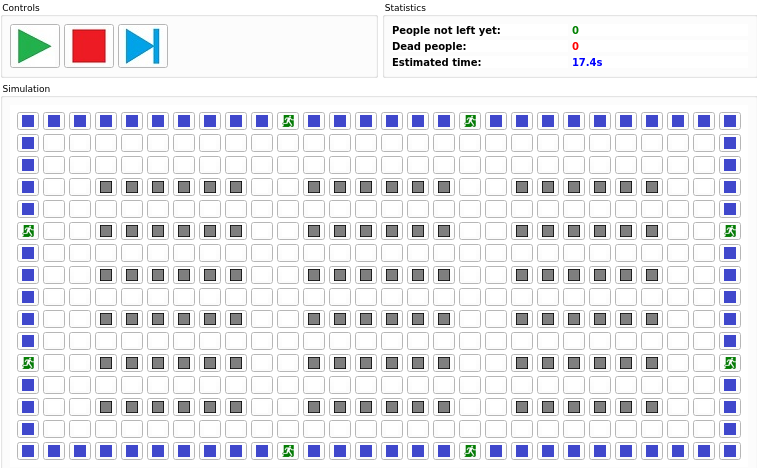
\includegraphics[width=8cm]{ExitDistribution/ExitDistribSevenEnd}
            \caption{Rozložení východů se šesti východy}
            \label{testExits7}
        \end{figure}

    \subsection{Hledání optimálního rozložení východů s~přítomností ohně}
    Tato část experimentů hledá dobrá rozložení východů z~hlediska bezpečnosti v~případě požáru. Bude-li například v~místnosti jen jeden východ a požár vznikne hned vedle něj, riziko úmrtí osob bude velmi vysoké.

        \subsubsection{Špatný příklad rozložení}
        Experiment ukazuje pohyb osob po místnosti v~situaci, kdy vznikl požár hned vedle jediného východu. Experiment používá výchozí parametry simulace. Obrázek~\ref{badFire} vlevo ukazuje počáteční stav simulace a vpravo ukazuje její výsledek. Jak jde vidět byl východ brzy pohlcen plameny a většina osob tak zůstala uvězněna v místnosti.\\

        \begin{figure}[H]
            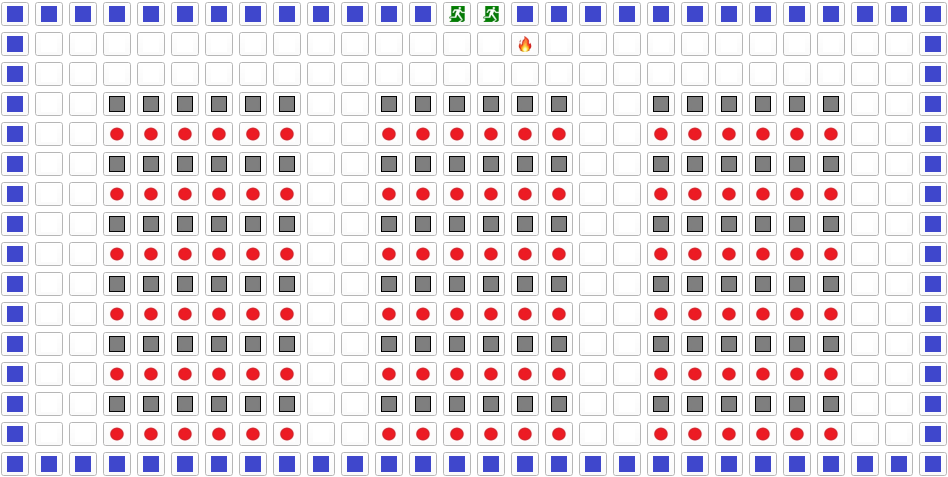
\includegraphics[width=8cm]{FireResearch/badFireInit}
            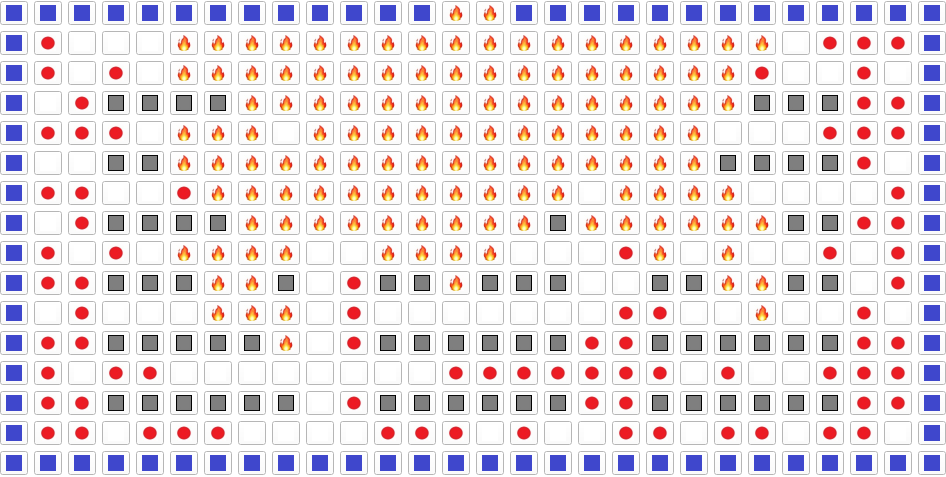
\includegraphics[width=8cm]{FireResearch/badFireEnd}
            \caption{Špatný příklad rozložení východů v~případě požáru}
            \label{badFire}
        \end{figure}

        \subsubsection{Východy na dvou stranách}
        Experiment ukazuje pohyb osob po místnosti, která má dva východy na protějších stranách. Experiment používá výchozí parametry simulace. Obrázek~\ref{goodFire} vlevo ukazuje počáteční stav simulace a vpravo ukazuje její výsledek. Oproti předchozímu experimentu je vidět, že přidání jednoho východu na opačnou stranu místnosti je velmi přínosné.\\

        \begin{figure}[H]
            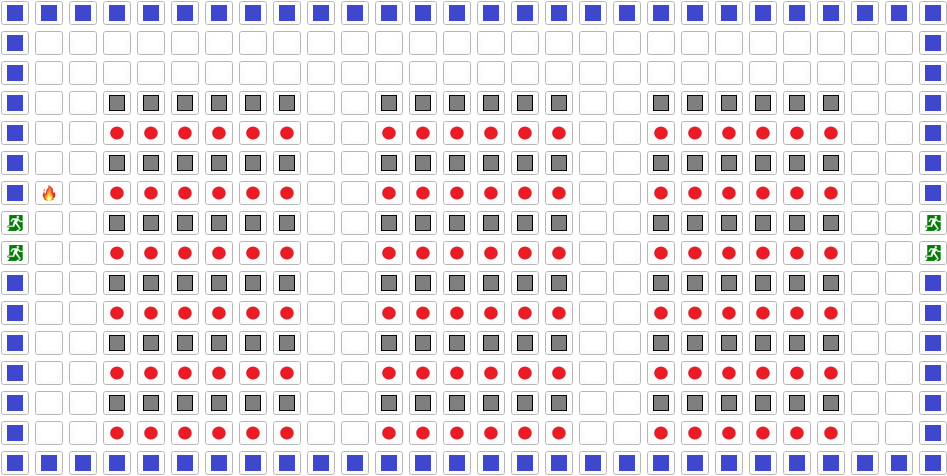
\includegraphics[width=8cm]{FireResearch/goodFireInit}
            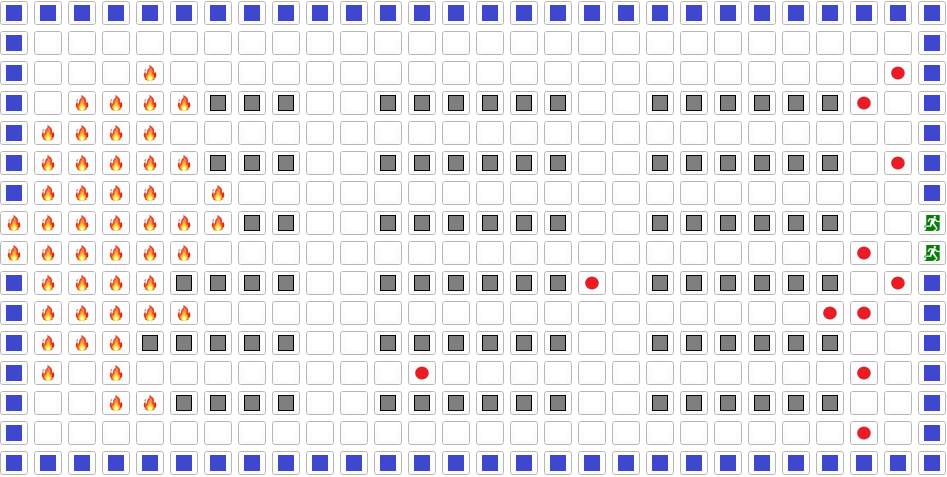
\includegraphics[width=8cm]{FireResearch/goodFireEnd}
            \caption{Dva východy na protějších stranách v~případě požáru}
            \label{goodFire}
        \end{figure}

        \subsubsection{Východy na třech stranách}
        Experiment ukazuje pohyb osob po místnosti, která má tři východy na různých stranách. Experiment používá výchozí parametry simulace. Obrázek~\ref{overFire} vlevo ukazuje počáteční stav simulace a vpravo ukazuje její výsledek. Oproti předchozímu experimentu proběhla celková evakuace rychleji. Z~hlediska požární bezpečnosti ale přidání třetího východu příliš nepřináší. Vzplanutí dvou východů současně je velmi nepravděpodobné a přínosy třetího východu nejspíše nepřevažují úsilí potřebné pro jeho přidání.\\

        \begin{figure}[H]
            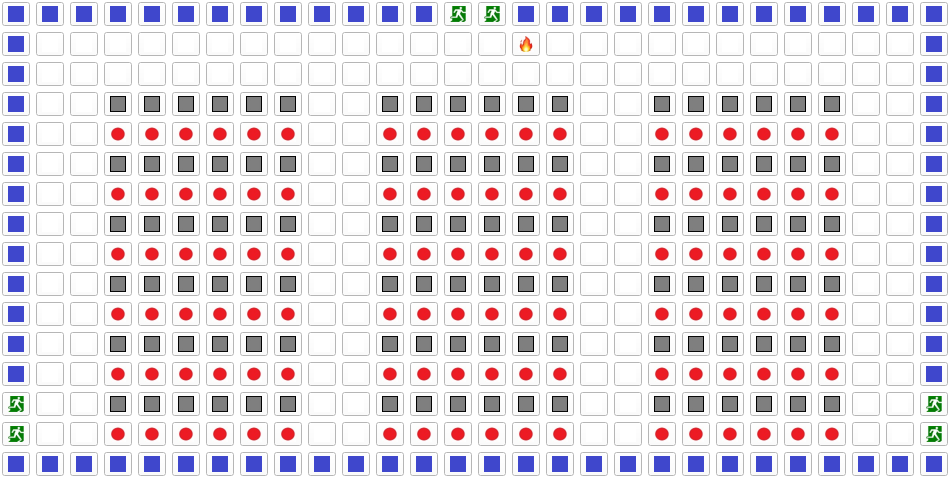
\includegraphics[width=8cm]{FireResearch/overFireInit}
            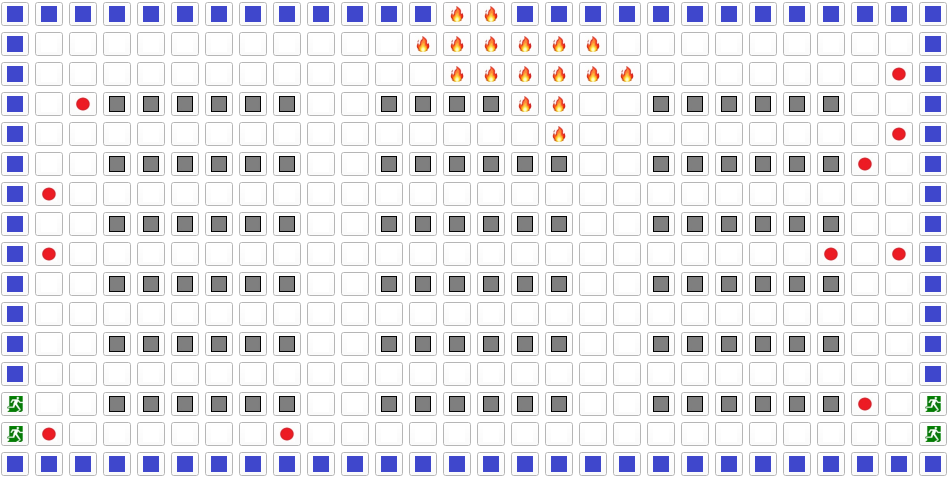
\includegraphics[width=8cm]{FireResearch/overFireEnd}
            \caption{Tři východy na různých stranách v~případě požáru}
            \label{overFire}
        \end{figure}

    \subsection{Závěr experimentů}
    Bylo provedeno minimálně 10 testovacích experimentů pro ověření funkčnosti a validity simulačního nástroje. Tyto experimenty ukazují funkčnost jednotlivých vlivů na pohyb osob v~simulaci. Všechny vlivy vykazují očekávaný efekt a lze tedy usuzovat, že jejich základní koncept je implementován správně a jsou do jisté míry validní. Testovací experimenty odhalily především chybu způsobenou lineární indexací pole buněk při výpočtu, která byla opravena procházením pole v~náhodném pořadí. Stále měnící se částí modelu jsou počáteční parametry simulace a především dominantnost jednotlivých vlivů pohybu osob. Parametry simulace je proto možné nastavit pomocí parametrů příkazové řádky při spouštění nástroje.

    Dále bylo provedeno 7 experimentů pro určení optimálního rozložení východů z~hlediska rychlosti evakuace. Jak bylo předpokládáno, nejlepší rozložení je rozložení s~velkým množstvím východů na všech stranách místnosti. Z~konstrukčního hlediska ale není možné, aby každá místnost měla téměř 10 východů. Proto pokládáme za nejvýhodnější~a nejoptimálnější~z hlediska zdrojů~a rychlosti evakuace architekturu se třemi východy, dva uprostřed řad sedadel~a jeden vzadu za diváky, aby nevznikala tzv. úzká hrdla~u dvou bočních východů~a lidé se netlačili~v uličkách. Při tomto rozložení východů je evakuace simulovaného prostoru možná za průměrně~29 sekund.

    Nakonec byly provedeny 3 experimenty zkoumající rozložení východů z~hlediska požární bezpečnosti. Jejich závěrem je, že pro eliminaci rizika uvíznutí osob kvůli odříznutí ohněm je potřeba mít v~místnosti alespoň dva východy na protějších stranách. Více východů na více stranách přispívá k~rychlosti evakuace, z~hlediska požární bezpečnosti ale již příliš nepřináší.

     

\section{Shrnutí simulačních experimentů a závěr}
    Výsledkem této simulační studie je simulační nástroj umožňující snadno modelovat různá rozložení východů z~místnosti kino sálu a experimentálně vyhodnocovat vlastnosti těchto rozložení. Simulační nástroj je podle testovacích experimentů dostatečně validní pro účel rychlého zkoušení různých rozložení východů. Cílem našich experimentů bylo, kromě ověření validity nástroje, nalézt nejefektivnější rozložení východů z~hlediska rychlosti evakuace a bezpečnosti v~případě požáru s~udržením počtu východů na minimum. Výsledky těchto experimentů jsou prezentovány a vysvětleny. Z~hlediska požární bezpečnosti je zásadní neshlukovat východy blízko sebe. Rychlost evakuace pak ne vždy roste se zvyšováním počtu východů, pokud nejsou správně rozmístěny.

\section{Bibliografie}

\begin{thebibliography}{2}
        
\bibitem{source_CA}
\textit{L.~Yang, K.~Zhu, S.~Liu; Cellular Automata Evacuation Model Considering Information Transfer in Building with Obstacles} [online]. [cit. 2018-11-28]. Dostupné z: \url{https://pdfs.semanticscholar.org/a11e/8c48634b954abd947eba1d1bcd67059dc5f6.pdf}

\bibitem{IMS}
\textit{P.~Peringer, M.~Hrubý; Prezentace předmětu IMS} [online]. [cit. 2018-11-28]. Dostupné z: \url{https://wis.fit.vutbr.cz/FIT/st/cfs.php?file=\%2Fcourse\%2FIMS-IT\%2Flectures&cid=12760}

\bibitem{walk_speed}
\textit{T.~Rinne, K.~Tillander, P.~Gronberg; Data collection and analysis of evacuation situations; kap.~4.4} [online]. [cit. 2018-11-28]. Dostupné z: \url{https://www.vtt.fi/inf/pdf/tiedotteet/2010/T2562.pdf}

\end{thebibliography}
        
\end{document}